\documentclass[../../book-main.tex]{subfiles}
\graphicspath{{\subfix{../..}}}

\begin{document}

\chapter{Consistent Representations via Autoencoding}
\label{ch:consistent}\label{ch:autoencoding}

\begin{quote}
  \hfill  ``{\em It has been obvious since the 1980s that
    backpropagation through deep autoencoders would be very effective
    for nonlinear dimensionality reduction, provided that computers
    were fast enough, data sets were big enough, and the initial
    weights were close enough to a good solution. All three conditions
  are now satisfied}.''

  $~$\hfill -- Geoffrey Hinton and Ruslan  Salakhutdinov, 2006
\end{quote}

\vspace{5mm}

%\yima{Autoencoding to ensure correctness and consistency: from PCA,
% dictionary learning to more general low-dimensional distributions,
% say mixture of low-dim subspaces and manifolds. Also from classical
% autoencoding with two separate, mutually inverse, mappings, to
% bidirectional mappings such as diffusion/denoising and sparse
% coding/decoding.}

In the past chapters, we have established a basic fact that the
fundamental goal of learning is to learn a data
distribution with low-dimensional supports and transform it to a compact and structured
representation. Such a representation reveals intrinsic
low-dimensional structures of the data distribution and facilitates
subsequent tasks such as classification and generation.

A fundamental approach to learning a good representation of such a
distribution is through {\em compression}. To make the
goal of compression measurable and computable, it can be done
explicitly by learning a coding scheme that minimizes the coding rate (entropy) or maximizes the information gain (coding rate
reduction). In this context, the fundamental role of a deep neural
network is to realize a certain iterative optimization algorithm that
incrementally optimizes the learned representations in terms of those measures:
\begin{equation}
  f\colon \X
  \xrightarrow{\hspace{1mm} f^0 \hspace{1mm}} \Z^0 \rightarrow \cdots
  \rightarrow \Z^\ell \xrightarrow{\hspace{1mm} f^\ell \hspace{1mm}}
  \Z^{\ell+1} \rightarrow  \cdots \to \Z^L = \Z.
\end{equation}
In the preceding chapter, we have shown that main architectural
characteristics of almost all popular deep networks (ResNet, CNN, and
Transformer) can be derived and interpreted from this perspective.

However, when we try to achieve a certain objective through
optimization, there is no guarantee that the solution $\Z$ found in
the end by incremental optimization is the correct solution. In fact, even if
the optimization process manages to find the globally optimal
solution $\Z^*$, there is no guarantee that the solution corresponds
to a complete representation of the data distribution.\footnote{This could be due to many reasons: for example, the data available for learning the distribution might not be sufficient, or formulation of the optimization program fails to consider some additional constraints or conditions.} Therefore, an outstanding question is how we can ensure that the learned representation of the data distribution is
correct or good enough. Of course, the only way to verify this is to
see whether there exists a decoding map, say $g$, that can decode the
learned representation to reproduce the original data (distribution)
well enough:
\begin{equation}
  \X
  \xrightarrow{\hspace{1mm} \mathcal{E} = f \hspace{1mm}} \Z
  \xrightarrow{\hspace{1mm} \mathcal{D} = g \hspace{1mm}} \hat{\X}
\end{equation}
in terms of some measure of similarity:
\begin{equation}
  d(\X, \hat \X).
\end{equation}
This leads to the concept of {\em autoencoding} that integrates the
encoding and decoding processes, which we have briefly alluded to in
Chapter \ref{ch:intro} (see Figure \ref{fig:autoencoder}) and have
studied some important special cases in Chapter \ref{ch:classic}. In
this chapter, Sections \ref{sec:consistent-representation} and
\ref{sec:NLPCA}, we will first study how to extend autoencoding to
more general classes of distributions via the principle of parsimony and consistency.

Of course, a fundamental motivation why we ever want to identify the
low-dimensional structures in a data distribution and find a good
representation is to make it easy to use the data for various tasks
of intelligence, such as classification, completion, and prediction.
Therefore, the resulting joint representation $(\x, \z)$ must be
structured in such a way that is best suited for these tasks. In
Sections \ref{sec:MAE} and \ref{sec:conditioned-decoding}, we will
see how an autoencoding should be structured to facilitate
conditioned completion or generation in either the data domain $\x$
or the feature domain $\z$ or across both domains.

\section{Consistent Representations}\label{sec:consistent-representation}
%\yima{Rewrite this to state the mathematical problem clearly,
% including assumptions (e.g. sufficiency) and objectives. Discuss
% approximations or variants of the objective that are computable and
% implementable.}

Here we give a formal definition of consistent representations, which
are closely related to the concept of autoencoding. %\yima{Maybe we
% want to separate definitions for the two types of consistency:
% Sample wise versus distribution wise.}
\begin{definition}[Consistent Representations]\label{def:bidirectional_rep}
  Given data \(\vX\), an \textit{consistent representation} is a pair
  of functions \((f \colon \cX \to \cZ, g \colon \cZ \to \cX)\), such
  that the \textit{features} \(\vZ = f(\vX)\) are compact and
  structured, and the \textit{autoencoding} \[\hat{\vX} \doteq g(\vZ)
  = g(f(\vZ))\] is \textit{close} to \(\vX\) according to either the
  following two measures:
  \begin{enumerate}
    \item We say that it is \textit{sample-wise} consistent if \(\vX
      \approx \hat{\vX}\) in certain norm with high probability.
    \item We say that the representation is \textit{distributionally
      consistent} if \(\Law(\vX) \approx \Law(\hat{\vX})\).
  \end{enumerate}
\end{definition}
%\sdb{Connected to perception vs.\ distortion.}

Acute readers may have noticed that if we do not impose certain
requirements on the representation $\Z$ sought, the above problem has
a trivial solution: One may simply choose the functions $f$ and $g$
to be the identity map! Hence, the true purpose of seeking for an
autoencoding is to try to ensure that so obtained $\Z$ is both more
compact and more structured than $\X$. Firstly, for compactness, $\Z$
should better reveal the intrinsic low-dimensionality of $\X$.
Therefore, the representation should maximize a certain information
gain, say, measured by the rate reduction
\begin{equation}
  \Delta R(\Z)
\end{equation}
introduced in the previous chapter. Secondly, the main purpose of
learning a good representation of the data distribution is to
facilitate tasks that exploit the low-dimensionality of its
distribution. Hence, the distribution of $\Z$ should be better
structured. For example, the distribution of $\Z$ is piecewise linear
or Gaussian, and its components are largely incoherent or independent
etc. These independent components can represent different clusters or
classes and can also be easily used as conditions for decoding the
corresponding data $\x$.

From the definition of consistent representation, it requires that
the representation $\Z$ is sufficient to recover the original data
distribution $\X$ to some degree of accuracy. For sample-wise
consistency, a typical choice is to minimize the expected reconstruction error:
\begin{equation}
  d(\X, \hat \X) = \mathbb{E}[\|\X - \hat\X\|_2^2].
\end{equation}
For consistency in distribution, a typical choice is to minimize a
certain distributional distance such as the KL
divergence\footnote{Note that for distributions without common
  support, which is typical for degenerate distributions, KL divergence
  may not even be well-defined. In fact, much of the distribution
  learning literature is trying to address this technical difficulty by
  replacing or approximating it with something well-defined and
efficiently computable.}:
\begin{equation}
  d(\X, \hat \X) = \mathcal{D}_{KL}(\X\|\hat\X).
\end{equation}

Hence, computation aside, when we seek a good autoencoding for a data
distribution $\X$,  conceptually we try to find an encoder $f$ and
decoder $g$ such that
\begin{equation}
  \min_{f, g} - \Delta R(\Z) + d(\X, \hat \X).
  \label{eqn:autoencode-objective-ch5}
\end{equation}
%\sdb{Maximize $\Delta R$?}
For the rest of this chapter, we will study how to solve such
autoencoding problems under different conditions, from simple and
ideal cases to increasingly more challenging and realistic conditions.

\section{From Linear to Nonlinear Autoencoding}\label{sec:NLPCA}
%\yima{How to ensure the representation is compact and structured,
% say linear or piecewise linear, or informative? Classical
% autoencoders do not explicitly impose such... Incremental
% flattening transformation, particularly
% \href{https://arxiv.org/abs/2305.01777}{nonlinear manifold
% flattening and reconstruction}. This is an example of consistency
% in sample-wise reconstruction.}

\subsection{Linear Autoencoding via PCA}
According to \cite{Baldi2011}, the phrase ``autoencoder'' was first
introduced by Hinton and Rumelhart \cite{Rumelhart1986} so that a
deep representation can be learned via back propagation (BP) in a self-supervision fashion---reconstructing the original data is the self-supervising task.

However, the very same concept of seeking a compact and consistent
representation has been rooted in
many classic studies. As we have already seen in Chapter
\ref{ch:classic}, the classical PCA, ICA, and sparse Dictionary
Learning all share a similar goal. The
only difference is when the underlying data distribution is simple (linear and
independent), the encoding or decoding mappings become easy to represent and
learn: they do not need to be deep and often can be computed in closed form or
with an explicit algorithm.

It is instructive to see how the notion of consistency we have
defined plays out in the simple case of PCA:
here, the consistent encoding and decoding mappings are given by a single-layer
linear transform:
\begin{equation}
  \X \xrightarrow{\hspace{2mm} \mathcal{E} = \vU^\top \hspace{2mm}}
  \Z \xrightarrow{\hspace{2mm} \mathcal{D} = \vU \hspace{2mm}}   \hat{\X},
  \label{eqn:autoencoding-PCA-2}
\end{equation}
where $\vU \in \mathbb{R}^{D\times d}$ typically with $d\ll D$. Hence
$\vU^\top $ represents a projection from a higher-dimensional space
$\mathbb{R}^{D}$  to a lower one $\mathbb{R}^{d}$, as illustrated in
Figure \ref{fig:AE}.
\begin{figure}
  \centering 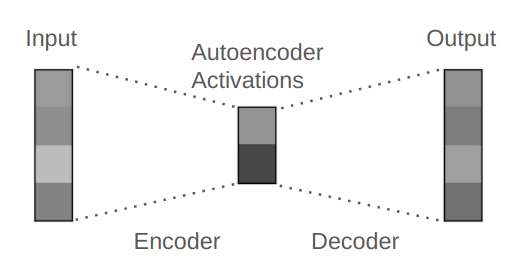
\includegraphics[width=0.5\linewidth]{figs_chap5/autoencoder.png}
  \caption{Illustration of a typical autoencoder such as PCA, seeking
  a low-dimensional representation $\bm{z}$ of high-dimensional data $\vx$.}
  \label{fig:AE}
\end{figure}

As we saw in Chapter \ref{ch:classic}, when the distribution of $\vx$ is indeed
supported on a low-dimensional subspace $\vU_o$, the compactness of
the representation
$\vz$ produced by $\cE$ is a direct consequence of correctly
estimating (and enforcing) the dimension of this subspace.  Finally,
recall that gradient descent on the reconstruction criterion exactly
yields these sample-wise consistent mappings: indeed, the optimal
solution to the problem
\begin{equation}\label{eq:pca-reconstruction-ch5}
  \min_{\vU \,\mid\, \vU^\top \vU = \vI}\, \bE_{\vx}\left[\norm*{\vx
  - \vU\vU^\top \vx}_2^2\right]
\end{equation}
precisely coincides with $\vU_o$ when the dimension of the representation is
sufficiently large. In this case, we obtain sample-wise consistency
for free, since this guarantees that $\vU_o\vU_o^\top \vx = \vx$.
Notice that in the case of PCA, the rate reduction term in
\eqref{eqn:autoencode-objective-ch5} becomes void as the regularization
on the representation $\Z$ sought is explicit: It spans the entire
subspace of lower dimension\footnote{One may view $\Delta R = 0$ in this case.}.

\paragraph{Online PCA.} Notice that in the above construction, the
linear transform $\vU$
used for the encoding and decoding is computed ``offline'' from all
the input data before hand. One question is whether this transform
can be learned ``online'' as the input data come in order? This
question was answered by the work of Oja in 1982 \cite{Oja1982SimplifiedNM}.
\begin{example}[Normalized Hebbian learning scheme for PCA] Consider a
  sequence of i.i.d. random vectors $\x_1, \ldots, \x_i, \ldots \in
  \mathbb{R}^n$ with covariance $\boldsymbol{\Sigma} \in
  \mathbb{R}^{n\times n}$. Let $\vu_0 \in \mathbb{R}^n$ and define
  the response of an input vector $\x_i$ against a weight vector
  $\vu_i$ to be their inner product:
  \begin{equation}
    \eta_i = \vu_i^T \x_i
  \end{equation}
  and we update the weight vector according to the following scheme:
  \begin{equation}
    \vu_{i+1} = \frac{\vu_i + \gamma \eta_i \x_i}{\|\vu_i + \gamma
    \eta_i \x_i\|}
    \label{eqn:Hebbian}
  \end{equation}
  for some small gain $\gamma >0$. This update scheme can be viewed
  as a normalized Hebbian scheme, in which the weights of connections
  between neurons become stronger if (products of) both the input
  $\x$ and output $\eta$ are strong. One may view the vector of
  weights $\vu$ are ``learned'' based on a form of feedback from the
  output $\eta$.
  Then, under reasonable assumptions, Oja \cite{Oja1982SimplifiedNM} has 
  shown that $\vu_i$ converges to the eigenvector associated with
  the large eigenvalue of $\boldsymbol{\Sigma}$.
\end{example}

The normalized Hebbian scheme \eqref{eqn:Hebbian} can be interpreted as
a first-order approximation to a \textit{stochastic} projected
gradient descent scheme on
the objective of the problem \eqref{eq:pca-reconstruction-ch5} (with batch size
$1$, and with the number of columns of $\vU$ equal to $1$) as long as
$\norm{\vu}_2 = 1$, which is maintained by the projection operation in
\eqref{eqn:Hebbian}.
It is worth keeping its existence in the back of one's mind, both as
a proof of correctness for the use of stochastic gradient methods for
optimizing reconstruction costs such as
\eqref{eq:pca-reconstruction-ch5}, and for its
suggestion that \textit{simpler algorithms than (end-to-end) back
  propagation can
succeed in learning consistent autoencoders}.

\begin{figure}
  \centering
  % \includegraphics[width=12cm]{interpolate.jpg}
  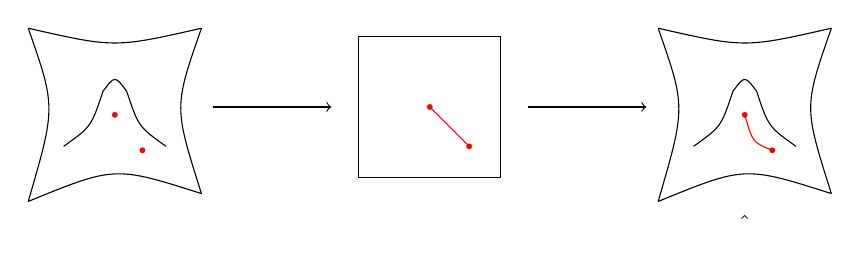
\begin{tikzpicture}
    \draw (-0.1, -0.2) .. controls (1, 0.25) .. (2.1, -0.1);
    \draw (2.1, -0.1) .. controls (1.75, 1) .. (2.1, 2);
    \draw (2.1, 2) .. controls (1, 1.75) .. (-0.1, 2);
    \draw (-0.1, 2) .. controls (0.25, 1) .. (-0.1, -0.2);

    \draw (0.35, 0.5) .. controls (0.7, 0.75) .. (0.85, 1.2);
    \draw (0.85, 1.2) .. controls (1.0, 1.4) .. (1.15, 1.2);
    \draw (1.15, 1.2) .. controls (1.3, 0.75) .. (1.65, 0.5);

    \node[fill, red, circle, inner sep=0.75pt] at (1, 0.9) {};
    \node[fill, red, circle, inner sep=0.75pt] at (1.35, 0.45) {};

    \node at (1, -0.5) {\(\x\)};

    \draw[->] (2.25, 1) -- (3.75, 1);
    \node at (3, 1.25) {\(\fl\)};

    \draw (4.1, 0.1) -- (5.9, 0.1);
    \draw (5.9, 0.1) -- (5.9, 1.9);
    \draw (5.9, 1.9) -- (4.1, 1.9);
    \draw (4.1, 1.9) -- (4.1, 0.1);

    \node[fill, red, circle, inner sep=0.75pt] at (5, 1) {};
    \node[fill, red, circle, inner sep=0.75pt] at (5.5, 0.5) {};

    \draw[red] (5, 1) -- (5.5, 0.5);

    \node at (5, -0.5) {\(\z\)};

    \draw[->] (6.25, 1) -- (7.75, 1);
    \node at (7, 1.25) {\(\re\)};

    \draw (7.9, -0.2) .. controls (9, 0.25) .. (10.1, -0.1);
    \draw (10.1, -0.1) .. controls (9.75, 1) .. (10.1, 2);
    \draw (10.1, 2) .. controls (9, 1.75) .. (7.9, 2);
    \draw (7.9, 2) .. controls (8.25, 1) .. (7.9, -0.2);

    \draw (8.35, 0.5) .. controls (8.7, 0.75) .. (8.85, 1.2);
    \draw (8.85, 1.2) .. controls (9.0, 1.4) .. (9.15, 1.2);
    \draw (9.15, 1.2) .. controls (9.3, 0.75) .. (9.65, 0.5);

    \node[fill, red, circle, inner sep=0.75pt] at (9, 0.9) {};
    \node[fill, red, circle, inner sep=0.75pt] at (9.35, 0.45) {};

    \draw[red] (9, 0.9) .. controls (9.1, 0.55) .. (9.35, 0.45);

    \node at (9, -0.5) {\(\hat{\x}\)};
  \end{tikzpicture}
  \caption{A depiction of interpolation through manifold flattening
    on a manifold in \(\R^{3}\) of dimension \(d = 2\). To interpolate
    two points on the data manifold, map them through the flattening
    map \(\fl\) to the flattened space, take their convex interpolants,
    and then map them back to the data manifold through the
  reconstruction map \(\re\).}
  \label{fig:idealized_interpolation}
\end{figure}

\subsection{Nonlinear PCA}\label{sub:nonlinear-pca}
Of course, one should expect that things will no longer be so simple
when we deal with more complex distributions whose underlying
low-dimensional structure could be nonlinear.

\paragraph{Data on a Nonlinear Submanifold.} So, to move beyond the
linear structure addressed by PCA, we may assume that the data distribution lies on a (smooth) submanifold $\mathcal{M}$. The intrinsic dimension of the submanifold, say $d$, is typically much lower than the
dimension of the ambient space $\mathbb{R}^D$. From this geometric
perspective, we typically want to find a nonlinear mapping $f$ such that
the resulting manifold
$f(\mathcal{M})$ is flattened, as illustrated by the example shown in Figure
\ref{fig:idealized_interpolation}. The resulting feature $\vz$-space
is typically
more compact (of lower-dimension) than the $\vx$-space, and the
manifold is flat.
From the statistical perspective, which is complementary to the geometric
perspective but distinct in general, we may also want to ensure that the data
distribution on $\cM$ is mapped to a sufficiently regular
distribution, say a Gaussian or a uniform distribution (with a 
very low-dimensional support), in the $\vz$-space. These two properties ensure that sampling and interpolation in the $\vz$-space are as easy as possible, and they are mathematical formalizations of the desirable
notions of compact and structured features in the low-dimensional manifold
model for the data distribution.
In general, the problem of learning such an autoencoding mapping for this class
of data distributions is known as {\em nonlinear principal component analysis}
(NLPCA).

\paragraph{A Classical Attempt via a Two-Layer Network.} As we have
seen above, in the case of PCA, a one-layer linear neural
network is sufficient. That is no longer the case for NLPCA. In 1991, Kramer
\cite{Kramer1991NonlinearPC}  proposed to solve NLPCA by using a two-layer
neural network to represent the encoder mapping $f$ (or its inverse $g$) based
on the universal representation property of two-layer networks with sigmoid
activation:
\begin{equation}
  \z = \vW_2 \sigma(\vW_1\x +\vb),
\end{equation}
where $\sigma(\spcdot)$ is the sigmoid function:
\begin{equation}
  \sigma(x) = \frac{1}{1+ e^{-x}}.
\end{equation}
Cybenko \cite{Cybenko1989ApproximationBS} showed that functions of
the above form (with enough hidden nodes) can approximate any smooth
nonlinear function, say the encoder $f(\spcdot)$, to an arbitrary
precision. In particular, they can represent the flattening and reconstruction
maps for data distributions supported on (unions of) low-dimensional manifolds,
as in \Cref{fig:idealized_interpolation}. The overall architecture of the
original networks proposed by Kramer is illustrated in Figure \ref{fig:NLPCA}.
\begin{figure}[tb]
  \centering
  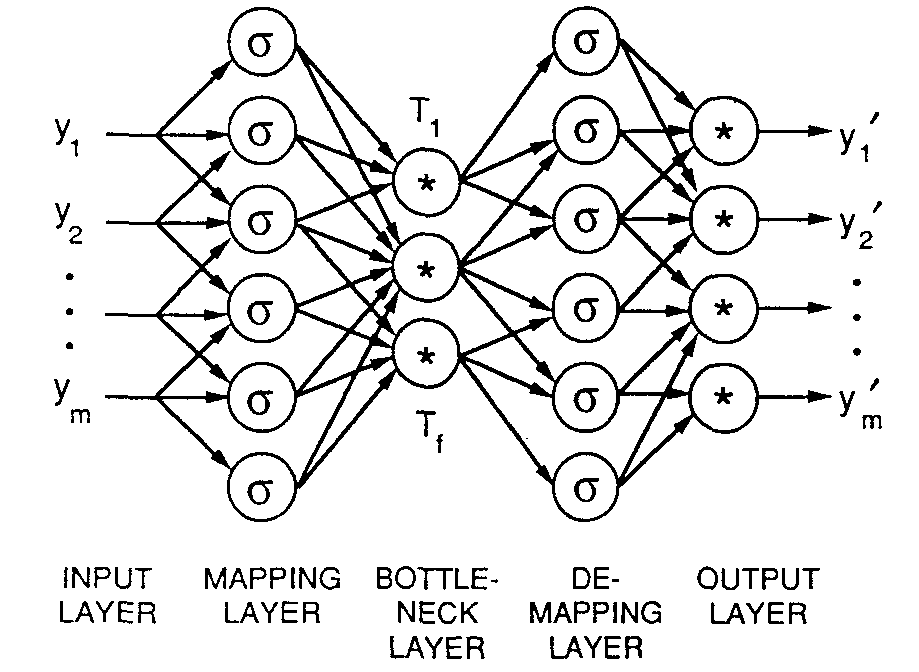
\includegraphics[width=0.6\linewidth]{figures/kramer1991nonlinearPCA.png}
  \caption{Nonlinear PCA by  autoassociative neural networks of depth
    two for both the encoding and decoding mappings, suggested by
  Kramer \cite{Kramer1991NonlinearPC}.}
  \label{fig:NLPCA}
\end{figure}

Unfortunately, unlike the above case of PCA, there is in general no
closed-form learning scheme for the parameters $\boldsymbol{\theta} =
(\vW, \vb)$ of these networks. Hence it was proposed to train the
network via back propagation with the supervision of reconstruction error:
\begin{equation}\label{eq:nonlinear-pca-ch5}
  \min_{\boldsymbol{\theta}} \mathbb{E}[ \|\x - \x'(\boldsymbol{\theta})\|^2].
\end{equation}
Compared to the simple case of PCA, we utilize the same reconstruction objective
for learning, but a far more complex nonlinear class of models for
parameterizing and learning the encoder and decoder. Although universal
approximation properties such as Cybenko's suggest that \textit{in principle}
learning consistent autoencoders via this framework is possible---because for
any random sample of data, given enough parameters, such autoencoding pairs
exist---one often finds it highly nontrivial to find them with gradient descent.
Moreover, to obtain an informative enough reconstruction objective
and model for the
distribution of high-dimensional real-world data such as images, the required
number of samples and hidden nodes can be huge.
In addition, as a measure of the compactness of the learned representation, the
(lower) dimension of $\z$ for the bottleneck layer is often chosen
heuristically.\footnote{In the later work \cite{Hinton-1993}, Hinton et.
  al. suggested to use the minimum description length (MDL) principle to promote
  the compactness of the learned coding scheme, in a spirit very similar to the
rate distortion measure introduced in this book.}
% \sdb{We can connect to Oja's here too: we learn with BP (don't just call GD)
% + it becomes nonlocal...}

\paragraph{Manifold Flattening via a Deeper Network.}
Based on the modern practice of deep networks, such classical shallow
and wide network architectures are known to be rather difficult to
train effectively and efficiently via back propagation (BP), partly
due to the diminishing gradient of the sigmoid function. Hence, the
modern practice normally suggests to further
decompose the nonlinear transform $f$ (or $g$) into a composition of
many more layers of simpler transforms, resulting a deeper network architecture
\cite{Hinton504}, as illustrated in Figure \ref{fig:ccnet_layers}.
In the modern context, further elaborations over the basic reconstruction cost
\eqref{eq:nonlinear-pca-ch5} also prove necessary to achieve good performance on
complex real-world data distributions such as images.

\begin{figure}[htb]
  \centering
  \begin{tikzpicture}
    \draw (-0.1, -0.2) .. controls (1, 0.25) .. (2.1, -0.1);
    \draw (2.1, -0.1) .. controls (1.75, 1) .. (2.1, 2);
    \draw (2.1, 2) .. controls (1, 1.75) .. (-0.1, 2);
    \draw (-0.1, 2) .. controls (0.25, 1) .. (-0.1, -0.2);

    \draw (0.35, 0.5) .. controls (0.7, 0.75) .. (0.85, 1.2);
    \draw (0.85, 1.2) .. controls (1.0, 1.4) .. (1.15, 1.2);
    \draw (1.15, 1.2) .. controls (1.3, 0.75) .. (1.65, 0.5);

    \node at (1, -0.5) {\(\x\)};

    \draw[->] (2.25, 1.25) -- (3.25, 1.25);
    \node at (2.75, 1.5) {\(\fl_{1}\)};

    \draw[->] (3.5, 1.25) -- (4.5, 1.25);
    \node at (4, 1.5) {\(\fl_{2}\)};

    \draw[->] (4.75, 1.25) -- (5.75, 1.25);
    \node at (5.25, 1.5) {\(\cdots\)};

    \draw[->] (6, 1.25) -- (7, 1.25);
    \node at (6.5, 1.5) {\(\fl_{L}\)};

    \draw[->] (7, 0.75) -- (6, 0.75);
    \node at (6.5, 0.5) {\(\re_{L}\)};

    \draw[->] (5.75, 0.75) -- (4.75, 0.75);
    \node at (5.25, 0.5) {\(\cdots\)};

    \draw[->] (4.5, 0.75) -- (3.5, 0.75);
    \node at (4, 0.5) {\(\re_{2}\)};

    \draw[->] (3.25, 0.75) -- (2.25, 0.75);
    \node at (2.75, 0.5) {\(\re_{1}\)};

    \draw (7.3, 0.1) -- (9.1, 0.1);
    \draw (9.1, 0.1) -- (9.1, 1.9);
    \draw (9.1, 1.9) -- (7.3, 1.9);
    \draw (7.3, 1.9) -- (7.3, 0.1);

    \node at (8.2, -0.5) {\(\z\)};

  \end{tikzpicture}
  \caption{A depiction of the construction process of the flattening
    and reconstruction pair \((\fl, \re)\), where the encoder \(\fl =
    \fl_{L} \circ \fl_{L - 1} \circ \cdots \circ \fl_{1}\) is
    constructed from composing flattening layers, and the decoder \(\re
    = \re_{1} \circ \re_{2} \circ \cdots \circ \re_{L}\) is composed of
  inversions of each \(\fl_{\ell}\).}
  \label{fig:ccnet_layers}
\end{figure}

In light of universal approximation theorems such as Cybenko's, one
may initially wonder why, conceptually, deeper autoencoders should be preferred
to shallow ones.
From purely an expressivity perspective, we can understand this phenomenon
through a geometric angle related to the task of flattening the nonlinear
manifold on which our hypothesized data distribution is supported. A purely
constructive approach to flattening the manifold proceeds incrementally, in
parallel to what we have seen in \Cref{ch:compression,ch:representation} with
the interaction between diffusion, denoising, and compression. In the geometric
setting, the incremental \textit{flattening process} corresponding to $f_{\ell}$
takes the form of transforming a neighborhood of one point of the manifold to be
closer to a flat manifold (i.e., a subspace), and enforcing local consistency
with the rest of the data samples; the corresponding incremental operation in
the decoder, $g_{\ell}$, undoes this transformation. This procedure precisely
incorporates curvature information about the underlying manifold, which is
estimated from data samples. Given enough samples from the manifold and
a careful instantiation of this conceptual process, it is possible to implement
this procedure as a computational procedure that verifiably flattens nonlinear
manifolds in a white-box fashion \cite{Psenka-JMLR24}. However, the approach is
limited in its applicability to high-dimensional data distributions such as
images due to unfavorable scalability, motivating the development of more
flexible methods to incremental autoencoding.

\subsection{Sparse Autoencoding}
In the above autoencoding schemes, the dimension of the feature space
$d$ is typically chosen to be much lower than that the original data
space $D$ so as to explicitly enforce or promote the learned
representation to be low-dimensional. However, in practice, we
normally do not know the intrinsic dimension of the data
distribution. Hence, the choice of the feature space dimension for
autoencoding is often done empirically. In more general situations,
the data distribution can be a mixture of a few low-dimensional
subspaces or submanifolds. In these cases, it is no longer feasible
to enforce a single low-dimensional space for all the features together.

The sparse autoencoder is meant to resolve some of these limitations. In
particular, the dimension of the feature space can be equal to or
even higher than that of the data space, as illustrated in Figure
\ref{fig:SAE}. However, the features are required to be highly
sparse in the feature space. So if we impose sparsity as the measure
of parsimony in addition to the rate reduction in the objective
\eqref{eqn:autoencode-objective-ch5}, we obtain a new objective for
the sparse autoencoding:
\begin{equation}
  \min_{f, g}
  %\lambda
  \|\Z\|_0 - \Delta R(\Z) + d(\X, \hat \X),
  \label{eqn:autoencode-sparse}
\end{equation}
where the $\ell^0$-``norm'' $\|\spcdot\|_0$ is known to promote sparsity.
This is very similar to the sparse rate reduction objective
\eqref{eq:sparse-rr} which we used in the previous Chapter \ref{ch:representation} to derive the white-box CRATE architecture.

\begin{figure}
  \centering
  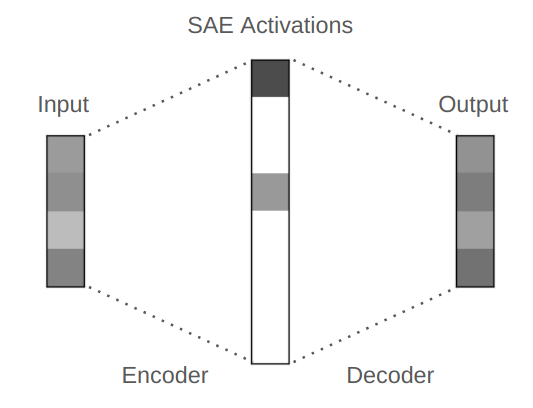
\includegraphics[width=0.5\linewidth]{figs_chap5/SAE_diagram.png}
  \caption{Illustration of a sparse autoencoder (SAE), compared to
  that of a typical autoencoder (AE) in Figure \ref{fig:AE}. }
  \label{fig:SAE}
\end{figure}

%\yima{There are other ways to promote the sparsity of the learned
% features $\Z$, including enforcing the frequency of activations for
%  each coordinate of $\z$ to be small... But here we can justify SAE
%  through its natural connection to sparse rate reduction. Anthropic
% AIseems to advocate that sparse autoencoding learns more
% interpretable features... }

As a method for learning autoencoding pairs in an end-to-end fashion, sparse
autoencoding has been practiced in the past \cite{Ranzato2006-oq}, but nearly
all modern autoencoding frameworks instead use a different, probabilistic
autoencoding framework, which we will study shortly.
However, it is worth noting that a significant amount of attention has been
devoted in recent years to training sparse autoencoders for the purpose of
\textit{interpreting features in pretrained large-scale deep networks}, such as
transformers, following the hypothesis that the (non-interpretable, \textit{a
priori}) features in these networks consist of sparse ``superpositions'' of
underlying features, which are themselves interpretable
\cite{elhage2022superposition}.
It is illuminating to contrast this methodology with the classical sparse
autoencoding framework, and with the general autoencoding methodology we have
laid out in this Chapter.
In the most straightforward instantiation of sparse autoencoder training and
evaluation (see \citep{huben2024sparse, gao2025scaling}),
a large number of features from a pretrained deep network $h$ are collected from
different inputs $\vx_i$, which themselves are chosen based on a desired
interpretation task.\footnote{For example, the inputs $\vx_i$ could correspond
  to texts containing samples of computer code in different
  programming languages,
  with our task being to try to identify interpretable features in a transformer
  feature map $h$ corresponding to different salient aspects of the
  input, such as
  the
  specific programming language (distinct across input ``classes'')
  or the need to
  insert a matching parenthesis at the current position (common
  across input ``classes''). We
  discuss the
  use of deep networks, and in particular transformers, for text representation
learning in greater detail in \Cref{ch:applications}.} For
simplicity, we will use $h$ to denote the pre-selected feature map in question,
with $D$-dimensional features; given $N$ sample inputs, let $\vH \in \bR^{D
\times N}$ denote the full matrix of features of $h$.
Then a sparse autoencoder $f : \bR^D \to \bR^d$, with decoder $g : \bR^d \to
\bR^D$, is trained via the relaxed version of the objective in
\Cref{eqn:autoencode-sparse}:
\begin{equation}\label{eq:sae-loss}
  \min_{f, g}
\lambda \|f(\vH)\|_1 + \frac{1}{2} \| \vH - g(f(\vH))) \|_2^2,
\end{equation}
where the sparse autoencoder $f$ commonly takes the form of a one-layer neural
network, i.e.\ $f(\vh_i) = \sigma(\vW_{\mathrm{enc}}(\vh_i - \vb)
+ \vb_{\mathrm{enc}})$, where $\sigma(x) = \max \{x, 0\}$ is the ReLU activation
function, and the decoder $g$ is linear, so that $g(\vz_i)
= \vW_{\mathrm{dec}}\vz + \vb$.
Interestingly, these simple architectures for the sparse autoencoder and decoder
can be seen as exactly analogous to those that would be obtained from the
unrolled optimization approach we have expounded in \Cref{ch:representation},
and in particular to the CRATE architecture's ISTA block
(\Cref{eq:grad_lasso_ista}).
More precisely, the sparse autoencoder's encoder can be seen as one step of
proximal gradient descent on the nonnegative LASSO objective, which, as we have
seen, leads to the CRATE ISTA block; the asymmetric structure of the encoder and
decoder can be similarly understood as the difference between the forward
mapping in the ISTA block (\Cref{eq:grad_lasso_ista}) and the sparsifying
dictionary $\vD$ itself, which becomes the decoder.
This connection suggests a host of new design strategies for improving the
representation ability of sparse autoencoders, few of which seem to have been
thoroughly explored thus far.

\subsection{Variational Autoencoding}

In the classical conception of autoencoding, following Hinton and Rumelhart
\cite{Rumelhart1986}, the data distribution plays a very minor role in the
formulation, in spite of its centrality to the representation we ultimately
learn. Indeed, in the naive framework, one hopes that by training a deep network
to reconstruct samples from the data distribution with a suitably-configured
bottleneck for the representation $\vz$, the learned encoders $f$ and $g$ will
naturally end up corresponding to a compact and structured feature
representation for the data. This is rarely the case in practice.
An improved, more modern methodology for autoencoding that still finds
significant application to this day is \textit{variational autoencoding}
\cite{Kingma2013-sb,Kingma2019-zh}.
We will see how this framework, which trains a variational autoencoder (VAE)
derived through probabilistic modeling considerations, both generalizes the
classical autoencoder training (via minimization of the reconstruction loss),
and stabilizes it with appropriate regularization. Later, we will see how to
begin to go further and go beyond the black-box nature of the deep networks used
to represent the encoding and decoding mappings $f$ and $g$.

\subsubsection{Probabilistic Perspective on Autoencoding}
In the manifold model for the data distribution, the key mathematical objects
are the \textit{support} of the data distribution, namely the manifold $\cM$,
and the density of the data on the support, say $p$. When we formulate
autoencoding from the probabilistic perspective, we often think of the
high-dimensional input $\vx$ as having a density $p$ with support on $\R^D$; one
can think of adding a very small amount of noise to the (degenerate)
distribution supported on the manifold $\cM$ to obtain this density $p$, in line
with our denoising-diffusion constructions in Chapter \ref{ch:compression}.
Then the goal of generative probabilistic modeling is to learn the density $p$
from samples $\vx$, say from a class of models $p(\vx;\, \vtheta)$ parameterized
by $\vtheta$. As we have recalled in Chapter \ref{ch:compression}, a classical
approach to achieving this is via maximum likelihood estimation:
\begin{equation*}\label{eq:VAE-MLE}
\max_{\vtheta}\, \bE_{\vx}[ \log p(\vx;\, \vtheta) ].
\end{equation*}
For certain representative classes of data distributions $p$ %
% , including the
% manifold model without any further geometric constraints
% \cite{kiani2024hardness},
and sufficiently-expressive classes of models $p(\vx;\, \vtheta)$, even simpler
learning problems than the maximum likelihood estimation problem are known to be
statistically hard \cite{Yang1999-wb}. Hence it is desirable to exploit the
knowledge that $\vx$ has low-dimensional structure by seeking to factor the
distribution $p(\vx ;\, \vtheta)$ according to a low-dimensional ``latent''
variable model $\vz$. Indeed, we may write by conditioning $p(\vx,
\vz ;\, \vtheta)
= p(\vz;\, \vtheta) p(\vx \mid \vz;\, \vtheta)$, and
\begin{align*}
p(\vx; \vtheta) &= \int p(\vz;\, \vtheta) p(\vx \mid \vz;\, \vtheta) \odif \vz
\\
&=
\bE_{\vz \sim p(\,\cdot\,;\, \vtheta)}[ p(\vx \mid \vz;\, \vtheta) ].
\end{align*}
Classically, our model for the data distribution $p(\vx;\, \vtheta)$ corresponds
to a choice of the latent distribution $p(\vz;\, \vtheta)$ and the conditional
distribution $p(\vx \mid \vz;\, \vtheta)$.
Even so, computing the model for the data distribution from these latent
distributions is intractable except for in special cases, analogous to those we
have studied in Chapter \ref{ch:classic}.
By the same token, computing the posterior $p(\vz \mid \vx;\, \vtheta)$ from
data, allowing us to \textit{encode} samples to their corresponding latents, is
generally intractable.
There is hence a tradeoff between the expressivity of our generative model,
its computational tractability, and the accuracy of any approximations we make
to the underlying probabilistic framework for the sake of
computational tractability.
In navigating this tradeoff, one also needs a flexible computational approach
for learning the model parameters $\vtheta$ from data, analogous to the maximum
likelihood objective.

In the variational autoencoding framework, we navigate this tradeoff through
three key insights:
\begin{enumerate}
\item We posit \textit{simple} distributions for $\vz$ and $\vx$ conditional
  on $\vz$, but make their parameters depend in a highly flexible way on the
  input data $\vx$ (where relevant) using deep networks.
\item We replace the posterior $p(\vz \mid \vx;\, \vtheta)$, used for encoding
  and whose form is implied (by Bayes rule) by our modeling choices for $\vz$,
  with a tractable approximation $q(\vz \mid \vx;\, \veta)$, which has its own
  parameters $\veta$.
\item We jointly learn $\vtheta$ and $\veta$ via maximizing a tractable lower
  bound for the likelihood $p(\vx ;\, \vtheta)$, known as the evidence lower
  bound (ELBO).
\end{enumerate}
We will focus on the most useful instantation of the VAE framework
for practice, namely
where the prior $p(\vz ;\, \vtheta)$ and the conditional $p(\vx \mid \vz;\,
\vtheta)$ are both Gaussian. Namely, we use the following Gaussian
distributions:
\begin{align*}
\vz &\sim \cN(\Zero, \vI), \\
\vx \mid \vz &\sim \cN(g_1(\vz), \diag(e^{g_2(\vz)}) \vI),
\end{align*}
where $g = (g_1, g_2)$ are deep networks with parameters $\vtheta$, which
correspond to the \textit{decoder} in the autoencoder.
Similarly, for the approximate posterior $q(\vz \mid \vx;\, \veta)$, we use
a special Gaussian distribution with parameters given by an encoder
MLP $f = (f_1, f_2)$ with parameters $\veta$:
\begin{equation*}
\vz \mid \vx \sim \cN(f_1(\vx), \diag(e^{f_2(\vx)}) \vI).
\end{equation*}
%\yima{We might need to elucidate what are the true implications of
% the above two assumptions on the forms of the two conditional
% distributions. How do these assumptions enforce certain desired
% structures of the representation and how are the structures related
% to what rate reduction and sparsity are promoting? }
This makes probabilistic encoding and decoding simple: we simply map our data
$\vx$ to mean and variance parameters of a Gaussian distribution for
encoding, or vice versa.
For learning the encoder and decoder, we start from the maximum likelihood
objective \Cref{eq:VAE-MLE}, and derive a convenient lower bound known as the
evidence lower bound, or ELBO. Starting from simple algebraic manipulations
\begin{align*}
\log p(\vx;\, \vtheta) &=
\log \frac{p(\vx, \vz;\, \vtheta)}{p(\vz \mid \vx;\, \vtheta)}
\\
&=
\log \frac{p(\vx, \vz;\, \vtheta)}{q(\vz \mid \vx;\, \veta)}
+
\log \frac{q(\vz \mid \vx;\, \veta)}{p(\vz \mid \vx;\, \vtheta)},
\end{align*}
we take expectations with respect to $\vz \sim q(\,\cdot\, \mid
\vx;\, \veta)$ and
use the Gibbs inequality (\Cref{thm:information-inequality}) to get
\begin{equation*}
\log p(\vx;\, \vtheta)
\geq
\bE_{\vz \sim q(\,\cdot\, \mid \vx ;\, \veta)} \left[
  \log \frac{p(\vx, \vz;\, \vtheta)}{q(\vz \mid \vx;\, \veta)}
\right].
\end{equation*}
The righthand side of this bound is the ELBO; as a lower bound for the pointwise
log-likelihood of $p(\vx;\, \vtheta)$, its maximization offers a
principled compromise
between the maximum likelihood objective and computational tractability.
Interestingly, the derivation above shows that its tightness depends on the KL
divergence between the approximate posterior $q(\vz \mid \vx;\, \veta)$ and the
true posterior $p(\vz \mid \vx;\, \vtheta)$, implying that the more accurate our
approximate posterior is, the more maximization of the ELBO leads to
maximization of the underlying objective of interest, the likelihood of the
data. Thus, the VAE objective is:
\begin{equation}\label{eq:elbo-objective}
\max_{\vtheta, \veta}\,
\bE_{\vx}
\bE_{\vz \sim q(\,\cdot\, \mid \vx ;\, \veta)} \left[
  \log \frac{p(\vx, \vz;\, \vtheta)}{q(\vz \mid \vx;\, \veta)}
\right].
\end{equation}
By our derivation, maximization of this objective corresponds to a tradeoff
between maximizing the likelihood function of the data and minimizing the KL
divergence between the approximate and true posterior, which is a highly
sensible objective given the VAE modeling assumptions.

\subsubsection{VAE Training as Probabilistic Autoencoding}

There is a general methodology for maximizing the ELBO objective in
\Cref{eq:elbo-objective} using stochastic gradient descent and various tractable
Monte Carlo estimators for the associated gradients. However, the task is
simpler under the Gaussian assumptions we have made above. In this case, the
ELBO reads
\begin{align*}
&\max_{\vtheta, \veta}\,
\bE_{\vx}
\bE_{\vz \sim q(\,\cdot\, \mid \vx ;\, \veta)} \left[
  \log \frac{p(\vx, \vz;\, \vtheta)}{q(\vz \mid \vx;\, \veta)}
\right]\\
=&
\max_{\vtheta, \veta}\,
\left\{
  \bE_{\vx}
  \bE_{\vz \sim q(\,\cdot\, \mid \vx ;\, \veta)} \left[
    \log p(\vx, \vz;\, \vtheta)
  \right]
  + \frac{d \log(2\pi e)}{2}
  % + \frac{1}{2}\sum_{i=1}^d f_{2, i}(\vx)
  + \frac{1}{2} \ip{ \bE_{\vx}[f_2(\vx)]}{\mathbf{1}}
\right\}
\\
\equiv &
\max_{\vtheta, \veta}\,
\left\{
  \bE_{\vx}
  \bE_{\vz \sim q(\,\cdot\, \mid \vx ;\, \veta)} \left[
    \log p(\vx \mid \vz;\, \vtheta)
    + \log p(\vz)
  \right]
  % +
  % \bE_{\vz \sim q(\,\cdot\, \mid \vx ; \veta)} \left[
  %   \log p(\vz)
  % \right]
  % + \frac{1}{2}\sum_{i=1}^d f_{2, i}(\vx)
  + \frac{1}{2} \ip{ \bE_{\vx}[f_2(\vx)]}{\mathbf{1}}
\right\}
\\
\equiv &
\max_{\vtheta, \veta}\,
\left\{
  2\bE_{\vx}\left[
    \bE_{\vz \sim q(\,\cdot\, \mid \vx ;\, \veta)} \left[
      \log p(\vx \mid \vz;\, \vtheta)
    \right]
    + \ip{ f_2(\vx) - e^{f_2(\vx)}}{\mathbf{1}}
    - \norm{f_1(\vx)}_2^2
    % + \frac{1}{2}\sum_{i=1}^d \left(
    %   f_{2, i}(\vx) - f_{1, i}^2(\vx) - e^{f_{2, i}(\vx)}
    % \right)
  \right]
\right\}, \labelthis \label{eq:elbo-for-gaussians}
\end{align*}
following the Gaussian entropy calculation done in
\Cref{app:diffusion-denoising}, \Cref{rem:gaussian-maxent}, where $\equiv$
denotes equivalence of optimization objectives (in each case, we remove some
additive constants that do not change the optimization problem's solutions).
The remaining term corresponds to the ``autoencoding'' part of the ELBO
objective: intuitively, it seeks to maximize the likelihood of data generated by
the decoder when the latents $\vz$ are distribited according to the approximate
posterior (generated by the encoder applied to a data sample $\vx$), which is
a probabilistic form of autoencoding.
To see this more directly, consider the special case where the approximate
posterior concentrates on its mean $f_1(\vx)$, for every $\vx$: this
is the limit
where its log-variance $f_{2,i}(\vx) \to -\infty$ for each coordinate
$i = 1, \dots, d$.
For simplicity, assume moreover that $g_2(\vx) = \mathbf{1}$, giving the decoder
constant unit variance on each coordinate.
Then the loss term in question converges to
\begin{align*}
\bE_{\vx}
\bE_{\vz \sim q(\,\cdot\, \mid \vx ;\, \veta)} \left[
  \log p(\vx \mid \vz;\, \vtheta)
\right]
&\to
\bE_{\vx} \left[
  \log p(\vx \mid f_1(\vx);\, \vtheta)
\right]
\\
% &=
% -\frac{1}{2} \bE_{\vx} \left[
%   (\vx - g_1\circ f_1(\vx))^\top \diag(e^{g_2\circ
% f_1(\vx)})^{-1} (\vx - g_1
%   \circ f_1(\vx))
%   % + \logdet\left( 2\pi \diag(e^{g_2 \circ f_1(\vx)}) \right)
%   + \sum_{i=1}^D (g_2 \circ f_1)_i(\vx)
% \right].
&\equiv
-\frac{1}{2} \bE_{\vx} \left[
  \|\vx - g_1\circ f_1(\vx)\|_2^2
\right].
\end{align*}
So with a highly confident encoder, which deterministically maps each sample
$\vx$ to a single point $f_1(\vx)$ in $\vz$-space, and an isotropic decoder,
the ``autoencoding'' part of the ELBO maximization problem indeed becomes
a classical autoencoding objective!\footnote{In the general case where $g_2$ is
not fixed as $\mathbf{1}$, the reader can verify that the autoencoding term in
the ELBO objective converges to a \textit{regularized} classical autoencoding
objective.}
At the same time, note that this special case is actually excluded by the
extra terms in \Cref{eq:elbo-for-gaussians}---these effectively correspond to
regularization terms that discourage the encoder from collapsing.
The general ELBO loss (\Cref{eq:elbo-objective,eq:elbo-for-gaussians}) is
therefore a strict generalization of the classical autoencoding reconstruction
objective (\Cref{eq:nonlinear-pca-ch5}), both in terms of its data fidelity term
and in terms of the inclusion of regularization terms.

\subsubsection{Training a VAE}
VAEs are typically trained by alternating stochastic gradient ascent on the ELBO
objective (\Cref{eq:elbo-for-gaussians}), given individual samples
$\vx$ from the
true data distribution and from $\vz \sim q(\,\cdot\,\mid \vx;\, \veta)$. In
particular, it is standard to collect and train on many independently-generated
samples $\vz^{i}$ for each sample $\vx$. To take gradients of
\Cref{eq:elbo-for-gaussians} with respect to the encoder parameters $\veta$,
one makes use of the so-called reparameterization trick by writing $\vz \sim
q(\,\cdot\,\mid \vx;\, \veta)$ as
\begin{equation*}
\vz =_{\mathrm{d}} f_1(\vx) + \diag(e^{\tfrac{1}{2}f_2(\vx)}) \vg,
\quad \vg \sim
\cN(0, \vI),
\end{equation*}
where $=_{\mathrm{d}}$ denotes equality in distribution. Then one can simply
take many independent standard Gaussian samples $\vg^{i}$ for each data sample
$\vx$, generate the corresponding samples from the approximate posterior
$\vz^i$, and compute gradients with respect to $\veta$ using automatic
differentiation without any issues.

\section{Data Completion via Masked Autoencoding}
\label{sec:MAE}
As we have alluded to at the beginning of the chapter, a good autoencoding should enable us to utilize the learned distribution of the data and its representation $(\x,\z)$ for various
estimation and generation tasks under different conditioning schemes.
The fundamental purpose of autoencoding is indeed to grant certain access to and \textit{control} over the distribution of the data. In the previous sections, we have developed the methodology of autoencoding in an abstract,
distribution-agnostic fashion. Here onwards, we will tailor our discussion
towards specific modern applications where we desire to learn useful
representations for specific structured data distributions, such as images, 3D
scenes, and videos, and where we have \textit{a priori} knowledge of certain
structured attributes of the data, such as class labels, text captions, or
physical poses, for which we would like to learn an autoencoding. In such cases, the modern practice is to establish such an autoencoding indirectly: rather than a direct encoder-decoder mapping between $\vx$ and $\vz$, we seek to establish a \textit{binding} via the joint distribution $(\vx, \vz)$, which grants us the ability to generate samples of $\vx$ conditioned on
the (specified \textit{a priori}) attributes $\vz$, or even to generate these
attributes conditioned on a data sample $\vx$. This methodology is highly
related to the direct encoder-decoder autoencoding loops we have discussed so
far in the Chapter,\footnote{And even uses it as a primitive in many cases, as
we will see, such as in the use of VAEs with conditional diffusion models.} but
it enables far more impressive applications, including all of the groundbreaking
multimodal capabilities of modern generative models.

In this Section, we will discuss how to exploit such an autoencoding
representation for completion tasks in the data domain: a pedagogically-useful special case of
the general binding formalism. More precisely, we study how to exploit the
(compressive) autoencoding for completing a data sample conditioned on a partial
observation of the data. We leave the study of data sampling and generation
conditioned on features or general observations to the next Section
\ref{sec:conditioned-decoding}.
Notice that in the setting we have discussed in previous Sections, the
autoencoding network is trained to reconstruct a set of complete samples of the
random vector $\x$. This would allow us to generate samples of the learned
(low-dimensional) distribution. In practice, however, the
low-dimensionality of the distribution is often exploited for
prediction or completion tasks. More specifically, we often need to
recover a sample  $\x$ when parts of it are missing (or even
corrupted). That is, we want to recover or predict the rest of $\x$
from observing only a fraction of it:
\begin{equation}
f: \mathcal{P}_{\Omega}(\x) \mapsto \hat{\x},
\end{equation}
where $\mathcal{P}_{\Omega}(\spcdot)$ represents a masking operation
(\Cref{fig:matrix-completion}).
\begin{example}[Classification] One may view the problem of
classification as a special case for completing or predicting
missing parts of a random vector. For classification, given a
sample vector $\x$, we would like to predict its class label $\y$.
If we stack the two together as one joint vector:
\begin{equation}
  \vw = (\x, \y),
\end{equation}
one may view the problem of predicting the class label $\y$ as a
problem of completing $\vw$ by observing only the $\x$ part. This
is usually done by estimating and transforming the joint
distribution of $\vw$ that minimizes the entropy (or coding
rate) of the resulting representation of the empirical distribution
of $\vx$.\footnote{A set of samples for $\x$ and their associated
class labels $\y$} In fact, the common practice of introducing an
auxiliary ``class token'' in the training of a Transformer for
classification tasks can be viewed as learning such a
representation by compressing (the coding rate of) given samples of
$\vw$. If the distribution of the data $\x$ is already a
mixture of (low-dimensional) Gaussians, the work
\cite{wright2008classification} showed that classification can be
done effectively by directly minimizing {\em the (lossy) coding
length} associated with the given samples.
\end{example}

\subsection{Matrix Completion}
Another classical problem of this kind is the low-rank {\em matrix
completion} problem. Consider a random vector $\x \in \mathbb{R}^m$
which is distributed according to a low-rank Gaussian (or
low-dimensional subspace) of rank $r < m$. Suppose we have drawn $n >
r$ independent samples from this distribution and form a matrix $\X =
[\x_1, \ldots, \x_n] \in \mathbb{R}^{m\times n}$. Obviously, the rank
of the matrix is
\begin{equation}
\mbox{rank}(\X) = r < \min\{m, n\}.
\end{equation}
Now let $\Omega$ indicate a set indices of observed entries of the
matrix $\X$. Let the observed entries to be:
\begin{equation}
\Y = \mathcal{P}_{\Omega}(\X).
\end{equation}
The remaining entries supported on $\Omega^c$ are unobserved or
missing. The problem is whether we can recover from $\Y$ the missing
entries correctly.  Figure \ref{fig:matrix-completion} shows one
example of matrix completion.
% \begin{figure}
%     \centering
%     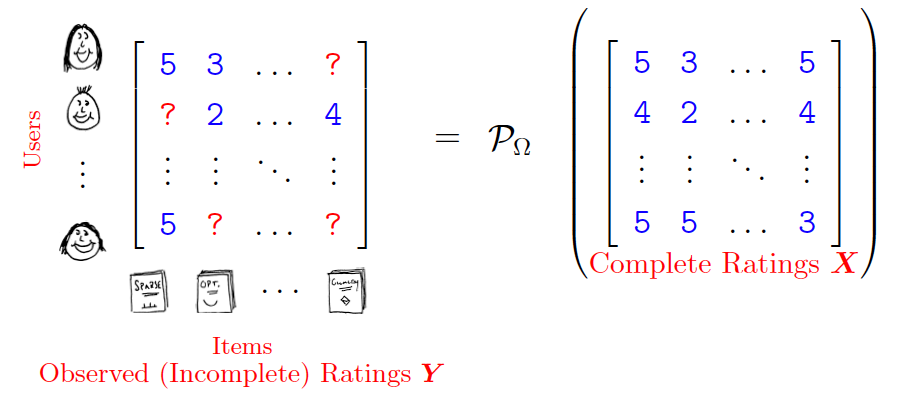
\includegraphics[width=0.8\linewidth]{figures/Matrix-Completion.png}
%     \caption{An example for completing a matrix with correlations
% among entries.}
%     \label{fig:matrix-completion}
% \end{figure}

\begin{figure}
\centering
% 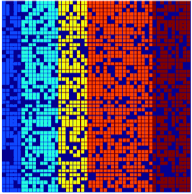
\includegraphics[width=0.3\linewidth]{figures/Matrix-masked.png}
% \hspace{5mm}  \hspace{5mm}
% 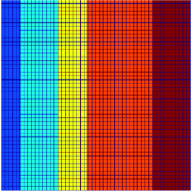
\includegraphics[width=0.3\linewidth]{figures/Matrix-completed.png}
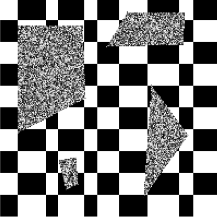
\includegraphics[width=0.3\linewidth]{figs_chap5/masked-checkerboard.png}\;\;
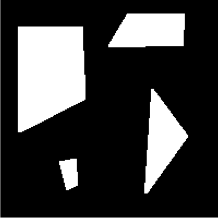
\includegraphics[width=0.3\linewidth]{figs_chap5/mask.png}\;\;
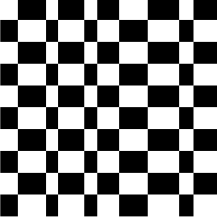
\includegraphics[width=0.3\linewidth]{figs_chap5/checkerboard.png}
\caption{Illustration of  completing an image as low-rank matrix
  with some entries masked or corrupted. Left: the masked/corrupted
image $\Y$; middle: the mask $\Omega$; right: the completed image $\hat \X$.}
\label{fig:matrix-completion}
\end{figure}

Notice that the fundamental reason why such a matrix can be completed
is because columns and rows of the matrix are highly correlated and
they all lie on a low-dimensional subspace. For the example shown in
Figure \ref{fig:matrix-completion}, the dimension or the rank of the
matrix completed is only two. Hence the fundamental idea to recover
such a matrix is to seek a matrix that has the lowest rank among all
matrices that have entries agreeing with the observed ones:
\begin{equation}
\min \mbox{rank}(\X) \quad \mbox{subject to}
\quad
\Y = \mathcal{P}_{\Omega}(\X).
\label{eqn:rank-min}
\end{equation}
This is known as the {\em low-rank matrix completion} problem.
However, as the rank function is discontinuous and rank minimization
is in general an NP-hard problem, we often like to relax it with
something easier to optimize.

Based on our knowledge about compression from Chapter
\ref{ch:compression}, we could  promote the low-rankness of the
recovered matrix $\X$ by enforcing the lossy coding rate (or the
volume spanned by $\X$) of the data in $\X$ to be small:
\begin{equation}
\min R_\epsilon(\X) = \frac{1}{2} \log \det \left(\boldsymbol{I} +
\alpha  \X\X^\top \right) \quad \mbox{subject to}
\quad
\Y = \mathcal{P}_{\Omega}(\X).
\label{eqn:rate-min}
\end{equation}
The problem can viewed as a continuous relaxation of the above
low-rank matrix completion problem \eqref{eqn:rank-min} and it can be
solved via gradient descent. As one can show, the gradient descent
operator for the $\log\det$ objective is precisely minimizing a close
surrogate of the rank of the matrix $\X\X^\top$.

The rate distortion function is a nonlinear function, and its gradient
descent does not always guarantee finding the correct solution.
However, since the underlying structure sought for $\X$ is linear,
the rank function admits a rather effective convex relaxation: the
nuclear norm---the sum of all singular values of the matrix $\X$. As
shown in the compressive sensing literature, under fairly
broad conditions,\footnote{Typically, such conditions specify the
necessary and sufficient amount of entries needed for the completion
to be computationally feasible. These conditions have been
systematically characterized in \cite{Wright-Ma-2022}.} the matrix
completion problem \eqref{eqn:rank-min}
can be effectively solved by the following convex program:
\begin{equation}
\min \|\X\|_* \quad \mbox{subject to}
\quad
\Y = \mathcal{P}_{\Omega}(\X),
\label{eqn:nuclear-min}
\end{equation}
where the nuclear norm $\|\X\|_*$ is the sum of singular values of
$\X$. In practice, we often convert the above constrained convex optimization
program to an unconstrained one:
\begin{equation}
\min \|\X\|_*  + \lambda \|
\Y - \mathcal{P}_{\Omega}(\X)\|_F^2,
\label{eqn:nuclear-min-lagrangian}
\end{equation}
for some properly chosen $\lambda > 0$. Interested readers may refer to
\cite{Wright-Ma-2022} for how to develop algorithms  that can solve
the above programs  efficiently and effectively.
Figure \ref{fig:matrix-completion} shows a real example in which the
matrix $\hat \X$ is actually recovered by solving the above program.

It has been shown that for images (or more accurately textures) and 3D scenes
with low-rank structures, they can be very effectively completed via
solving optimization programs of the above kind, even if there is
additional corruption and distortion
\cite{Zhang2010TILTTI,Liang-ECCV2012,Yi_2023_ICCV}.

\subsection{Masked Autoencoding}
For a general image $\vX$ such as the one shown on the left of Figure
\ref{fig:crate_mae_pipeline}, we can no longer view it as a low-rank
matrix. However, humans still demonstrate remarkable ability to
complete a scene and recognize familiar objects despite severe
occlusion. This suggests that our brain has learned the
low-dimensional distribution of natural images and can use it for
completion, hence recognition. However, the distribution of all
natural images is not as simple as a low-dimensional linear subspace.
Hence a natural question is whether we can learn the more
sophisticated distribution of natural images and use it to perform
image completion?

\begin{figure}[t!]
%\vspace{-0.5in}
\begin{center}
  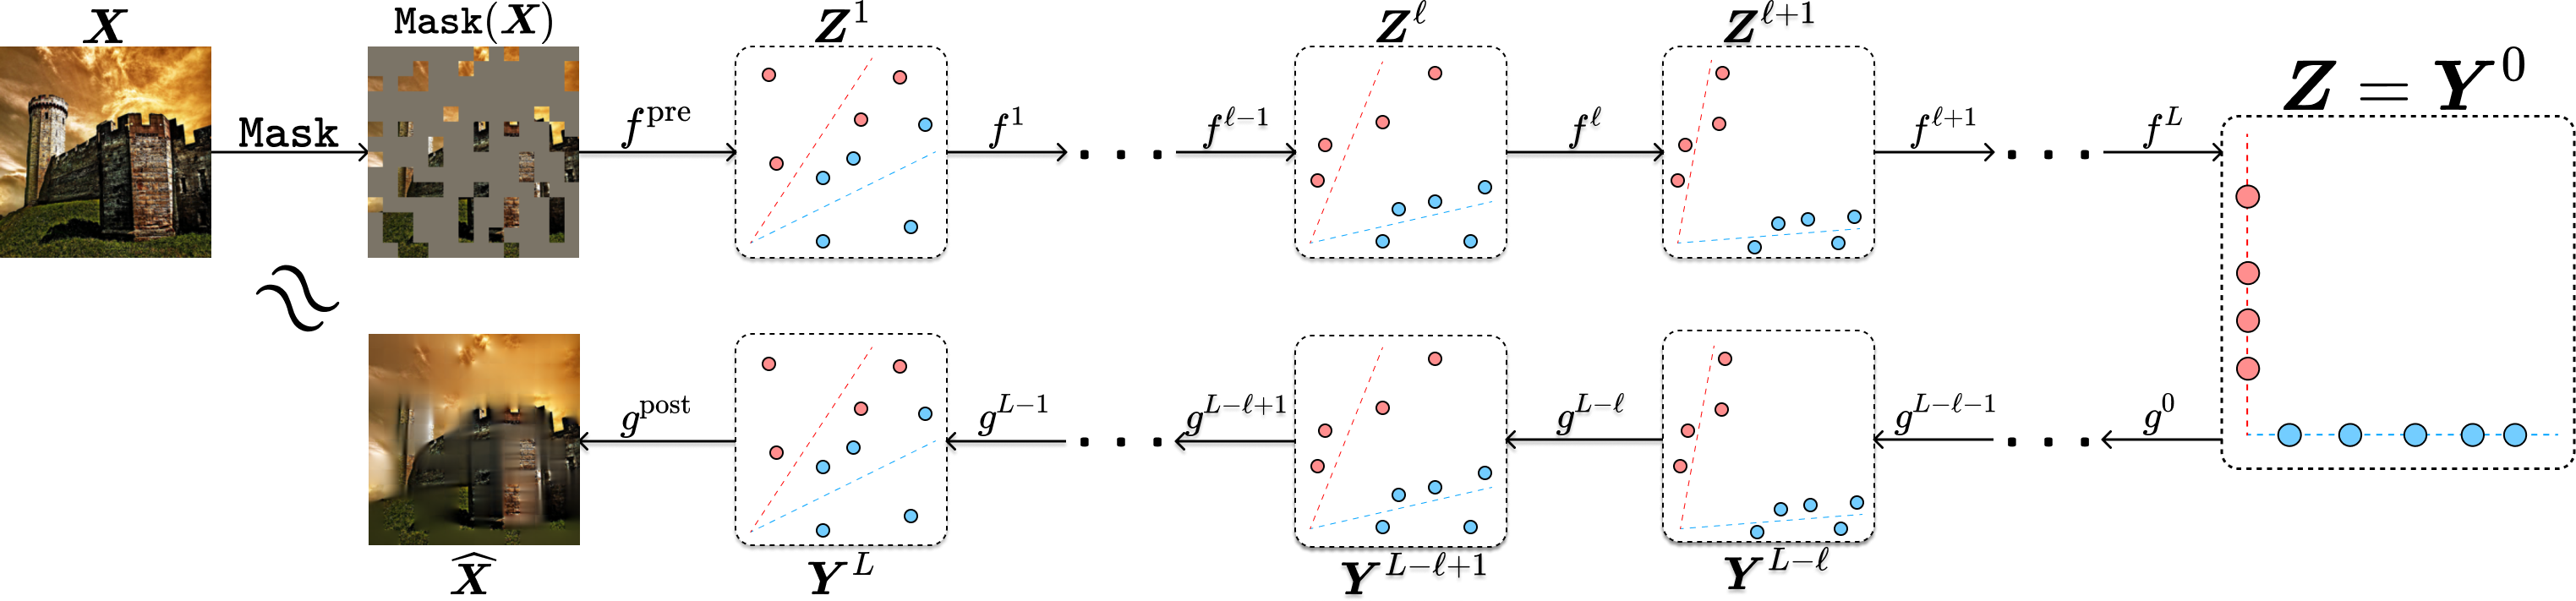
\includegraphics[width=0.99\textwidth]{figs_chap5/crate_mae_pipeline.png}
\end{center}
%\vspace{-0.1in}
\caption{\small \textbf{Diagram of the overall  (masked)
  autoencoding process.} The (image) token representations are
  transformed iteratively towards a parsimonious (e.g., compressed
  and sparse) representation by each encoder layer \(f^{\ell}\).
  Furthermore, such representations are transformed back to the
  original image by the decoder layers \(g^{\ell}\). Each encoder
  layer \(f^{\ell}\) is meant to be (partially) inverted by a
corresponding decoder layer \(g^{L - \ell}\).}
\label{fig:crate_mae_pipeline}
%\vspace{-0.2in}
\end{figure}

One natural approach is to find an encoding and decoding scheme by
solving the following {\em masked autoencoding} (MAE) program that
minimizes the reconstruction loss:
\begin{equation}\label{eq:mae_loss}
\min L_{\mathrm{MAE}}(f, g) \doteq \mathbb{E}\big[\norm{(g \circ
f)(\mathcal{P}_\Omega(\vX)) - \vX}_{2}^{2}].
\end{equation}
Unlike the matrix completion problem which has a simple underlying
structure, we should no longer expect that the encoding and decoding
mappings admit simple closed forms or the program can be solved by
explicit algorithms.

For a general natural image, we can no longer assume its columns or
rows are sampled from a low-dimensional subspace or a low-rank
Gaussian. However, it is reasonable to assume that the image consists
of multiple regions. Image patches in each region are similar and can
be modeled as one (low-rank) Gaussian or subspace. Hence, to exploit the low-dimensionality of the distribution,  the objective \textit{of the
encoder} $f$ is to transform $\X$ to a representation $\Z$ such that the distribution of $\Z$ can be well modeled as a mixture of subspaces, say $\{\vU_{[K]}\}$,
such that the overall coding rate and sparsity of the resulting
feature $\Z$ is the minimum:
\begin{equation}\label{eq:sparse_rr}
\min \mathbb{E}_{\vZ}[\Delta R(\vZ \mid \vU_{[K]}) - \lambda
\norm{\vZ}_{0}] = \mathbb{E}_{\vZ}[R(\vZ) - R^{c}(\vZ \mid
\vU_{[K]}) - \lambda \norm{\vZ}_{0}].
\end{equation}

As we have shown in the previous Chapter \ref{ch:representation}, the
encoder $f$ that minimizes the above objective can be constructed by
a sequence of transformer-like operators. As shown in the work of
\cite{Pai2024masked}, the decoder $g$ can be viewed and hence
constructed explicitly as the inverse process of the encoder $f$.
Figure \ref{fig:crate_mae_layers} illustrates the overall
architectures of both the encoder and the corresponding decoder at
each layer. The parameters of the encoder $f$ and decoder $g$ can be
learned by optimizing the reconstruction loss \eqref{eq:mae_loss} via
gradient descent.

\begin{figure}[t!]
%\vspace{-0.5in}
\centering
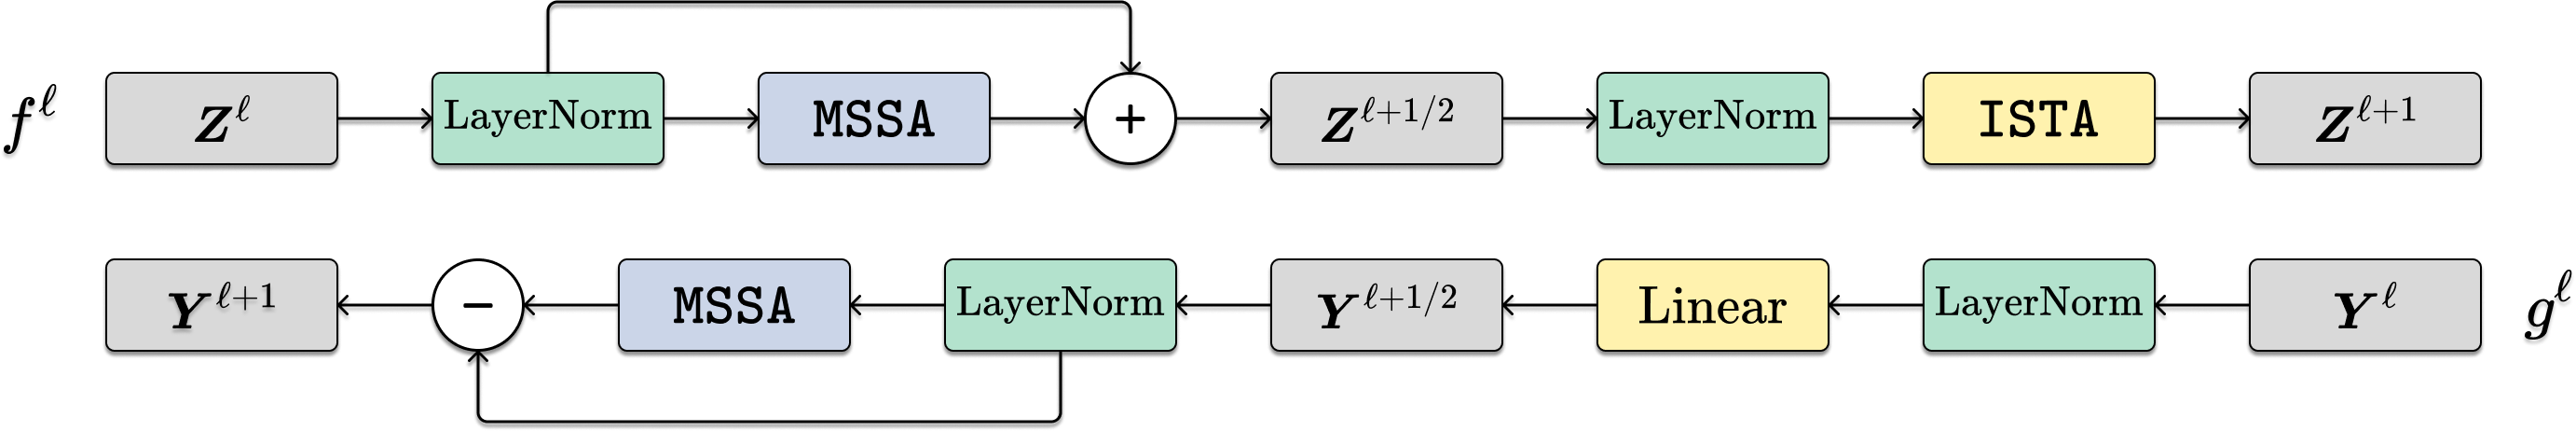
\includegraphics[width=0.99\textwidth]{figs_chap5/crate_mae_layers.png}
%\vspace{-0.1in}
\caption{\small \textbf{Diagram of each encoder layer
  (\textit{top}) and decoder layer (\textit{bottom}).} Notice that
  the two layers are highly anti-parallel --- each is constructed to
  do the operations of the other in reverse order. That is, in the
  decoder layer \(g^{\ell}\), the \(\ISTA\) block of \(f^{L - \ell}\)
  is partially inverted first using a linear layer, then the
  \(\MSSA\) block of \(f^{L - \ell}\) is reversed; this order
unravels the transformation done in \(f^{L - \ell}\).}
\label{fig:crate_mae_layers}
%\vspace{-0.2in}
\end{figure}

Figure \ref{fig:mae_autoencoding-small} shows some representative
results of the so-designed masked auto-encoder. More implementation details and
results of the masked autoencoder for natural image completion can be
found in Chapter \ref{ch:applications}.
\begin{figure}[t]
%\vspace{-0.5in}
\centering
\includegraphics[width=0.99\textwidth]{figs_chap5/crate_mae_autoencoding_small.pdf}
%\vspace{-0.1in}
\caption{\small \textbf{Autoencoding visualizations of CRATE-Base
  and ViT-MAE-Base \cite{he2022masked} with 75\% patches masked.}
  We observe that the reconstructions from CRATE-Base are on par
  with the reconstructions from ViT-MAE-Base, despite using \(<
  1/3\) of the parameters.
}
\label{fig:mae_autoencoding-small}
%\vspace{-0.2in}
\end{figure}

%\yima{Generalize low-rank matrix completion to masked autoencoding
% (MAE):  \href{https://arxiv.org/abs/2404.02446}{masked image completion}. }

%\yima{Maybe trying to optimize rate reduction type objective...
% Theoretical justification: maybe mention the recent work from Qing
% Qu's group about memorization and generalization (diffusion process
% for the PCA or mixture of low-dim Gaussians case). Probably some
% work on incremental optimal transport...}

%\section{Conditional Denoising and Diffusion}
%\label{sec:auto-denoising-diffusion}
%\yima{We now relax the requirement of sample-wise reconstruction to
% distribution-wise.}

\section{Conditional  Sampling of Denoising Models}
\label{sec:conditioned-decoding}
The above (masked) autoencoding problems can be viewed to sample the learned low-dimensional distribution such that the generated samples are consistent with certain observations or conditions.

But let us examine the image completion task studied in the previous
section: Given the
visual part of an image $\X_v = \mathcal{P}_{\Omega}(\X)$, we try to
estimate the masked part $\X_m = \mathcal{P}_{\Omega^c}(\X)$. For realizations
$(\vXi_v, \vXi_m)$ of the random variable $\vX=(\vX_v, \vX_m)$, let
\[p_{\X_m \mid \X_v}(\vXi_m\mid \vXi_v)\]
be the conditional distribution of $\X_m$ given
$\X_v$. It is easy to show that the optimal solution to the  MAE
formulation \eqref{eq:mae_loss} is given by the conditional expectation:
\begin{equation}
  \argmin_{h = g \circ f}\, L_{\mathrm{MAE}}(h)
  % \doteq \mathbb{E}\big[\norm{(g \circ f)(\mathcal{P}_\Omega(\vX)) - \vX}_{2}^{2}].
  = \vXi_v \mapsto \vXi_v + \mathbb{E}[\X_m \mid \X_v=\vXi_v].
\end{equation}
In general, however, this expectation may not even be on the
low-dimensional distribution of natural images! This partially
explains why some of the recovered patches in \Cref{fig:mae_autoencoding-small}
are a little blurry.

For many practical purposes, we would like to learn (a representation
of) the conditional distribution $p_{\X_m \mid \X_v}$, or equivalently
$p_{\X \mid \X_v}$,
and then sample this distribution directly. Notice that, when the
distribution of $\X$ is low-dimensional, it is possible that if a
sufficient part of $\X$, $\X_v$, is observed, it fully determines
$\X$ hence the missing part $\X_m$. In other words, the distribution
$p_{\X \mid \X_v}$ is a generalized function---if $\vX$ is fully determined by
$\vX_v$ it is the delta function, and more generally one of its exotic cousins.

\subsection{Conditional Sampling with Measurement
Matching}\label{sub:measurement-matching}
To generalize the above (image) completion problems, we may consider
that a random vector $\vx \sim p$ is partially observed through a more
general observation function:
\begin{equation}\label{eq:measurement-matching-observation}
\vy = h(\vx) + \vw,
\end{equation}
where $\vw$ usually stands for some random measurement noise, say of
a Gaussian distribution $\vw \sim \mathcal{N}(\mathbf{0}, \sigma^2
\boldsymbol{I})$. It is easy to see that, for so related $\x$ and $\y$, their joint distribution $p(\x, \y)$ is naturally nearly degenerate if the noise $\vw$ is small. To a large extent, we may view $p(\x, \y)$ as a noisy version of a hypersurface defined by the function $\y = h(\x)$ in the joint space $(\x, \y)$.  Practically speaking, we will consider a setting more akin to masked autoencoding than to pure matrix completion, where we always have access to a corresponding clean sample $\vx$ for every observation $\vy$ we receive.\footnote{In some more specialized applications, in particular in scientific imaging, it is of interest to be able to learn to generate samples
from the posterior $p_{\x \mid \y}$ without access to any clean/ground-truth samples of $\x$. We give a brief overview of methods for this setting in the
end-of-chapter notes.}

Like image/matrix completion, we
are often faced with a setting where $\vy$ denotes a degraded or otherwise
``lossy''
observation of the input $\vx$. This can manifest in quite different
forms. For example, in various scientific or
medical imaging problems, the measured data $\vy$ may be a compressed and
corrupted observation of the underlying data $\vx$; whereas in 3D vision tasks,
$\vy$ may represent an image captured by a camera of a physical object with an
unknown (low-dimensional) pose $\vx$.
Generally, by virtue of mathematical modeling (and, in some cases, co-design
of the measurement system), we know $h$ and can evaluate it on any input, and
we can exploit this knowledge to help reconstruct and sample $\vx$.

\begin{figure}[t]
  \centering
  \begin{subfigure}{0.45\textwidth}
    \vspace{0.75cm}
    \centering
    \begin{tikzcd}[column sep=1.5cm]
      \vx \arrow[r, "h(\vx) + \vw"] & \vy \arrow[r, "p_{\vx \mid \vy}"]
      & \posteriorsample \arrow[r, "\posteriorsample + t\vg"] & \posteriorsample_t
    \end{tikzcd}
    \vspace{0.75cm}
    \caption{}
    \label{fig:left}
  \end{subfigure}
  \hfill
  \begin{subfigure}{0.45\textwidth}
    \centering
    \begin{tikzcd}[column sep=1.5cm, row sep=0.5cm]
    & \vy \\
    \vx \arrow[ur, "h(\vx) + \vw"] \arrow[dr, "\vx + t\vg"] & \\
    & \vx_t
    \end{tikzcd}
    \caption{}
    \label{fig:right}
  \end{subfigure}
  \caption{Statistical dependency diagrams for the conditional sampling process.
  \textbf{Left:} In a direct (conceptual) application of the diffusion-denoising scheme
  we have developed in \Cref{ch:compression} to conditional sampling, we use
  samples from the posterior $p_{\vx \mid \vy}$ to train denoisers directly on
  the posterior at different noise levels, then use them to generate new
  samples. In practice, however, we do not normally have direct samples from the
  posterior, but rather paired samples $(\vx, \vy)$ from the joint.
  \textbf{Right:} It turns out that it suffices to have only noisy observations
  of $\vx$ to realize the denoisers corresponding to $p_{\posteriorsample_t \mid
  \posteriorsample}$: this follows from conditional independence of $\vx_t$ and
  $\vy$ given $\vx$. It implies that $p_{\posteriorsample_t} = p_{\vx_t \mid
  \vy}$, which gives a score function for denoising that consists of the
  unconditional score function, plus a correction term that enforces measurement
  consistency.}
  \label{fig:posterior-sampling-cds}
\end{figure}


At a technical level, we want the learned representation of the data
to facilitate us to sample the conditional distribution $p_{\vx\mid
\vy}$, also known as the posterior, effectively and efficiently. More precisely,
write $\vnu$ to denote a realization of the random variable $\vy$.
We want to generate samples $\hat{\x}$ such that:
\begin{equation}\label{eq:goal-sample-posterior}
  \hat{\x} \sim   p_{\vx \mid \y}(\spcdot \mid \vy=\vnu).
\end{equation}

Recall that in \Cref{sub:compression_denoising}, we have developed a natural and
effective way to produce \textit{unconditional} samples of the data distribution
$p$. The ingredients are the denoisers $\bar{\x}^\ast(t, \vxi) = \bE[ \x \mid
\vx_t=\vxi ]$, or their learned approximations $\bar{\x}_{\theta}(t, \vxi)$,
for different levels of noisy observations $\x_t = \x + t \vg$ (and $\vxi$ for
their realizations) under
Gaussian noise $\vg \sim \cN(\mathbf{0}, \vI)$, and $t \in
[0, T]$ with a choice of times $0 = t_1 < \hdots < t_{L} = T$ at which to
perform the iterative denoising, starting from $\hat{\vx}_{t_L} \sim
\cN(\mathbf{0}, T^2 \vI)$ (recall \Cref{eq:denoising-iteration-basic}).\footnote{Recall from our discussion in \Cref{sub:sampling_denoising}
that a few small improvements to this basic iterative denoising scheme are
sufficient to bring competitive practical performance. For clarity as we develop
conditional sampling, we will focus here on the simplest instantiation.}
We could directly apply this scheme to generate samples from the posterior
$p_{\vx \mid \vy}$ \textit{if} we had access to a dataset of samples
$\posteriorsample \sim p_{\vx \mid \y}(\spcdot \mid \vnu)$ for each realization
$\vnu$ of $\vy$, by generating noisy observations
$\posteriorsample_t$ and training denoisers to approximate $\bE[
  \posteriorsample \mid \posteriorsample_t=\spcdot, \vy=\vnu ]$, the mean of the posterior under
the noisy observation (see \Cref{fig:posterior-sampling-cds}(a)).
However, performing this resampling given only paired samples $(\vx, \vy)$ from the
joint distribution (say by binning the samples over values of $\vy$) requires
prohibitively many samples for high-dimensional data, and alternate approaches
explicitly or implicitly rely on density estimation, which similarly suffers from the
curse of dimensionality.

Fortunately, it turns out that this is not necessary.
Consider the alternate statistical dependency diagram in
\Cref{fig:posterior-sampling-cds}(b), which corresponds to the random variables
in the usual denoising-diffusion process, together with the measurement $\vy$. 
Because our assumed observation model \eqref{eq:measurement-matching-observation}
implies that $\vx_t$ and $\vy$ are independent conditioned on $\vx$, we have for
any realization $\vnu$ of $\vy$
\begin{align*}
  p_{\posteriorsample_t\mid \vy}(\spcdot \mid \vnu)
  &= \int
  \underbrace{p_{\posteriorsample_t \mid \posteriorsample}(\spcdot\mid \vxi)}_{=
  \cN(\vxi, t^2 \vI)}
  \spcdot \underbrace{p_{\posteriorsample \mid \vy}}_{= p_{\vx\mid \vy}}(\vxi \mid
  \vnu)
  \odif \vxi
  \\
  &=
  \int p_{\vx_t \mid \vx, \vy}(\spcdot\mid \vxi, \vnu) \spcdot p_{\vx \mid
  \vy}(\vxi\mid \vnu) \odif \vxi
  \\
  &=
  \int p_{\vx_t, \vx \mid \vy}(\spcdot, \vxi \mid \vnu) \odif \vxi
  \\
  &= p_{\vx_t \mid \vy}(\spcdot\mid \vnu).
\end{align*}
Above, the first line recognizes an equivalence between the distributions
arising in \Cref{fig:posterior-sampling-cds}(a, b); the second line applies this
together with conditional independence of $\vx_t$ and $\vy$ given $\vx$; the
third line uses the definition of conditional probability; and the final line
marginalizes over $\vx$.
Thus, the denoisers from the conceptual posterior sampling process are equal to
$\bE[\vx \mid \vx_t=\spcdot, \vy=\vnu]$, which we can learn solely from paired samples $(\vx,
\vy)$,
% and the posterior with respect to $\vx_t$ and $\vy$ can be expressed using
% Bayes' rule as
% \begin{equation}
%   p(\vx \mid \vx_t, \vy) = \frac{p(\vx_t \mid \vx) p(\vx \mid \vy)}{p(\vx_t \mid
%   \vy)},
% \end{equation}
% where we used that $\vx_t$ is an independent Gaussian conditional on $\vx$.
and by Tweedie's formula (\Cref{thm:tweedie}), we can express these denoisers in
terms of the score function of $p_{\vx_t \mid \vy}$, which, by Bayes' rule,
satisfies
\begin{equation}
  p_{\vx_t \mid \vy}(\vxi \mid \vnu) 
  = \frac{p_{\vy \mid \vx_t}(\vnu \mid \vxi) p_{\vx_t}(\vxi)}{p_{\vy}(\vnu)}.
\end{equation}
Recall that the density of $\vx_t$ is 
given by $p_t = \varphi_{t} \ast p$, where $\varphi_{t}$ denotes the standard
Gaussian density with zero mean and covariance $t^2 \vI$ and $\ast$ denotes
convolution. This is nothing but the \textit{unconditional score function}
obtained from the standard diffusion training that we developed in
\Cref{sub:compression_denoising}!
The conditional score function then satisfies, for any realization $(\vxi,
\vnu)$ of $(\vx_t, \vy)$,
\begin{equation}
  \nabla_{\vxi} \log p_{\vx_t \mid \vy}(\vxi\mid \vnu)
  =
  \underbrace{\nabla_{\vxi} \log p_t(\vxi)}_{\text{score matching}}
  +
  \underbrace{\nabla_{\vxi} \log p_{\vy \mid \vx_t}(\vnu \mid \vxi)}_{\text{measurement matching}},
\end{equation}
giving (by Tweedie's formula) our proposed denoisers as
\begin{align*}
  \bE[ \vx \mid \vx_t=\vxi, \vy=\vnu]
  &=
  \vxi + t^2 \nabla_{\vxi}\log p_t(\vxi) + t^2 \nabla_{\vxi}\log p_{\vy \mid
  \vx_t}(\vnu \mid \vxi)
  \\
  &=
  \bE[\vx \mid \vx_t=\vxi] + t^2 \nabla_{\vxi}\log p_{\vy \mid \vx_t}(\vnu\mid
  \vxi).
  \labelthis \label{eq:posterior-sampling-denoiser-decomposition}
\end{align*}
The resulting operators are interpretable as a \textit{corrected} version of the
unconditional denoiser for the noisy observation, where the correction term (the
so-called ``measurement matching'' term) enforces consistency with the
observations $\vy$. The reader should take care to note to which argument the
gradient operators are applying in the above score functions in order to fully
grasp the meaning of this operator.

The key remaining issue in making this procedure computational is to prescribe
how to compute the measurement matching correction, since in general we do not
have a closed-form
expression for the likelihood $p_{\vy \mid \vx_t}$ except for when $t
= 0$. Before taking up this problem, we discuss an illustrative concrete example
of the entire process, continuing from those we have developed in
\Cref{sub:compression_denoising}.

\begin{example}\label{example:denoising-conditional-gaussian}
  Consider the case where the data distribution is Gaussian with mean $\vmu \in
  \bR^D$ and
  covariance $\vSigma \in \bR^{D \times D}$, i.e., $\vx \sim \cN(\vmu, \vSigma)$.
  Assume that $\vSigma \succeq \Zero$ is nonzero.
  Moreover, in the measurement model \eqref{eq:measurement-matching-observation},
  suppose we obtain linear measurements of $\vx$ with independent Gaussian
  noise, where $\vA \in \bR^{d \times D}$ and $\vy = \vA \vx + \sigma \vw$
  with $\vw \sim \cN(\Zero, \vI)$ independent of $\vx$.
  Then $\vx =_{d} \vSigma^{1/2} \vg + \vmu$, where $\vg \sim \cN(\Zero, \vI)$ is
  independent of $\vw$ and $\vSigma^{1/2}$ is the unique positive square root of
  the covariance matrix $\vSigma$, and
  after some algebra, we can then write
  \begin{equation*}
    \begin{bmatrix}
      \vx \\
      \vy
    \end{bmatrix}
    =_{d}
    \begin{bmatrix}
      \vSigma^{1/2} & \Zero \\
      \vA \vSigma^{1/2} & \sigma \vI
    \end{bmatrix}
    \begin{bmatrix}
      \vg \\
      \vw
    \end{bmatrix}
    +
    \begin{bmatrix}
      \vmu \\
      \vA\vmu
    \end{bmatrix}.
  \end{equation*}
  By independence, we have that $(\vg, \vw)$ is jointly Gaussian, which means that
  $(\vx, \vy)$ is also jointly Gaussian, as the affine image of a jointly Gaussian
  vector.
  Its covariance matrix is given by
  \begin{equation*}
    \begin{bmatrix}
      \vSigma^{1/2} & \Zero \\
      \vA \vSigma^{1/2} & \sigma \vI
    \end{bmatrix}
    \begin{bmatrix}
      \vSigma^{1/2} & \Zero \\
      \vA \vSigma^{1/2} & \sigma \vI
    \end{bmatrix}^\top
    =
    \begin{bmatrix}
      \vSigma & \vSigma \vA^\top \\
      \vA \vSigma & \vA \vSigma \vA^\top + \sigma^2 \vI
    \end{bmatrix}.
  \end{equation*}
  Now, we apply the fact that conditioning a random vector with joint Gaussian
  distribution on a subset of coordinates is again a Gaussian distribution
  (\Cref{exercise:conditional_gaussian}).
  By this, we obtain that
  \begin{equation}
    p_{\x \mid \y}(\spcdot \mid \vnu) = \cN\left(
    \underbrace{%
      \vmu + \vSigma\vA^\top \left(\vA\vSigma\vA^\top + \sigma^2 \vI\right)^{-1} 
      (\vnu - \vA\vmu)}_{\vmu_{\vx \mid \vy}(\vnu)},
      \underbrace{%
      \vSigma - \vSigma \vA^\top \left(\vA\vSigma\vA^\top + \sigma^2
      \vI\right)^{-1} \vA \vSigma}_{\vSigma_{\vx\mid \vy}}
    \right).
  \end{equation}
  By the equivalence we have derived above, we get by another application of
  \Cref{exercise:conditional_gaussian}
  \begin{equation}\label{eq:conditional-posterior-denoiser-gaussian-case}
    \bE[ \vx \mid \vx_t=\vxi, \vy=\vnu ]
    =
    \vmu_{\vx\mid \vy}(\vnu) + \vSigma_{\vx\mid\vy}\left(
    \vSigma_{\vx\mid \vy} + t^2 \vI 
    \right)^{-1}\left(
    \vxi - \vmu_{\vx\mid \vy}(\vnu)
    \right).
  \end{equation}
  The functional form of this denoiser is quite simple, but it carries an
  unwieldy dependence on the problem data $\vmu$, $\vSigma$, $\vA$, and
  $\sigma^2$.
  We can gain further insight into its behavior by comparing it with
  \Cref{eq:posterior-sampling-denoiser-decomposition}.
  We have as usual
  \begin{equation}\label{eq:posterior-denoiser-gaussian-case}
    \bE[\vx \mid \vx_t=\vxi]
    = \vmu + \vSigma\left(\vSigma + t^2 \vI\right)^{-1} (\vxi - \vmu),
  \end{equation}
  which is rather simple---suggesting that the measurement matching term is
  rather complicated. To confirm this, we can calculate the likelihood $p_{\vy
  \mid \vx_t}$ directly using the following expression for the joint
  distribution of $(\vx_t, \vy)$:
  \begin{equation}
    \begin{bmatrix}
      \vx \\
      \vx_t \\
      \vy
    \end{bmatrix}
    =_{d}
    \begin{bmatrix}
      \vSigma^{1/2} & \Zero & \Zero \\
      \vSigma^{1/2} & t\vI & \Zero \\
      \vA \vSigma^{1/2} & \Zero & \sigma \vI
    \end{bmatrix}
    \begin{bmatrix}
      \vg \\
      \vg' \\
      \vw
    \end{bmatrix}
    +
    \begin{bmatrix}
      \vmu \\
      \vmu \\
      \vA\vmu
    \end{bmatrix},
  \end{equation}
  where $\vg' \sim \cN(\Zero, \vI)$ independent of the other Gaussians.
  This is again a jointly Gaussian distribution; restricting to only the final
  two rows, we have the covariance
  \begin{equation*}
    \begin{bmatrix}
      \vSigma^{1/2} & t\vI & \Zero \\
      \vA \vSigma^{1/2} & \Zero & \sigma \vI
    \end{bmatrix}
    \begin{bmatrix}
      \vSigma^{1/2} & t\vI & \Zero \\
      \vA \vSigma^{1/2} & \Zero & \sigma \vI
    \end{bmatrix}^\top
    =
    \begin{bmatrix}
      \vSigma + t^2\vI & \vSigma\vA^\top \\
      \vA\vSigma & \vA\vSigma\vA^\top + \sigma^2 \vI
    \end{bmatrix}.
  \end{equation*}
  Another application of \Cref{exercise:conditional_gaussian} then gives us
  \begin{equation}
    p_{\y \mid \vx_t}(\spcdot \mid \vxi) = \cN\left(
    \underbrace{%
      \vA\vmu + \vA\vSigma\left( \vSigma + t^2 \vI \right)^{-1}
      \left(
        \vxi - \vmu
      \right)
      }_{\vmu_{\vy \mid \vx_t}(\vxi)},
      \underbrace{%
        \vA\vSigma\vA^\top + \sigma^2 \vI - \vA\vSigma \left( \vSigma
        + t^2 \vI\right)^{-1} \vSigma \vA^\top
      }_{\vSigma_{\vy\mid \vx_t}}
    \right).
  \end{equation}
  Now notice that $\vmu_{\vy \mid \vx_t}(\vxi) = \vA \bE[\vx \mid \vx_t=\vxi]$.
  So, by the chain rule,
  \begin{align*}
    t^2 \nabla_{\vxi} \log p_{\vy \mid \vx_t}(\vnu \mid \vxi)
    &=
    t^2 \nabla_{\vxi}\left[
      -\frac{1}{2}
      (\vnu - \vA \bE[\vx \mid \vx_t=\vxi])^\top
      \vSigma_{\vy \mid \vx_t}^{-1}
      (\vnu - \vA \bE[\vx \mid \vx_t=\vxi])
      \right]
    \\
    &= t^2 (\vSigma+t^2 \vI)^{-1}\vSigma\vA^\top\vSigma_{\vy \mid \vx_t}^{-1}\left(
    \vnu - \vA \bE[\vx \mid \vx_t=\vxi] \right).
    \labelthis
    \label{eq:conditional-posterior-measurementmatching-gaussian-case}
  \end{align*}
  This gives us a more interpretable decomposition of the conditional posterior
  denoiser \eqref{eq:conditional-posterior-denoiser-gaussian-case}: following
  \Cref{eq:posterior-sampling-denoiser-decomposition}, it is the sum of the
  unconditional posterior denoiser \eqref{eq:posterior-denoiser-gaussian-case}
  and the measurement matching term
  \eqref{eq:conditional-posterior-measurementmatching-gaussian-case}.
  We can further analyze the measurement matching term. Notice that
  \begin{equation}
    \vSigma_{\vy \mid \vx_t}
    =
    \sigma^2 \vI + \vA\vSigma^{1/2} \left(
      \vI - \vSigma^{1/2}\left(
      \vSigma + t^2 \vI
      \right)^{-1}
      \vSigma^{1/2}
    \right)\vSigma\vA^\top.
  \end{equation}
  If we let $\vSigma = \vV \vLambda \vV^\top$ denote an eigenvalue decomposition
  of $\vSigma$, where $(\vv_i)$ are the columns of $\vV$, we can further write
  \begin{align}
    \vSigma^{1/2}\left(
    \vI - \vSigma^{1/2}\left(
    \vSigma + t^2 \vI
    \right)^{-1}
    \vSigma^{1/2}
    \right) \vSigma^{1/2}
    &=
    t^2 \vV \vLambda^{1/2}\left(
      \vLambda + t^2 \vI
    \right)^{-1}
    \vLambda^{1/2}
    \vV^\top
    \\
    &=
    t^2 \sum_{i=1}^D
    \frac{\lambda_i}{\lambda_i + t^2}
    \vv_i \vv_i\adj.
  \end{align}
  Then for any eigenvalue of $\vSigma$ equal to zero, the corresponding summand
  is zero; and
  writing $\lambda_{\min}(\vSigma)$ for the smallest positive eigenvalue of
  $\vSigma$ (it has at least one positive eigenvalue, by assumption), we have
  (in a sense that can be made quantitatively precise) that whenever $t \ll
  \sqrt{\lambda_{\min}(\vSigma)}$, it holds
  \begin{equation}
    \frac{\lambda_i t^2}{\lambda_i + t^2} \approx 0.
  \end{equation}
  So, when $t \ll \sqrt{\lambda_{\min}(\vSigma)}$, we have the approximation
  \begin{equation}
    \vSigma_{\vy \mid \vx_t} \approx \sigma^2 \vI.
  \end{equation}
  The righthand side of this approximation is equal to $\vSigma_{\vy \mid \vx}$.
  So we have in turn
  \begin{equation}
    \nabla_{\vxi} \log p_{\vy \mid \vx_t}(\vnu \mid \vxi)
    \approx
    \nabla_{\vxi} \log p_{\vy \mid \vx}(\vnu \mid \bE[\vx \mid \vx_t = \vxi]).
    \label{eq:conditional-posterior-measurementmatching-gaussian-case-dps-approx}
  \end{equation}

  \begin{figure}[tbp]
    \centering
    % Top row (3 images)
    \begin{subfigure}{0.32\textwidth}
      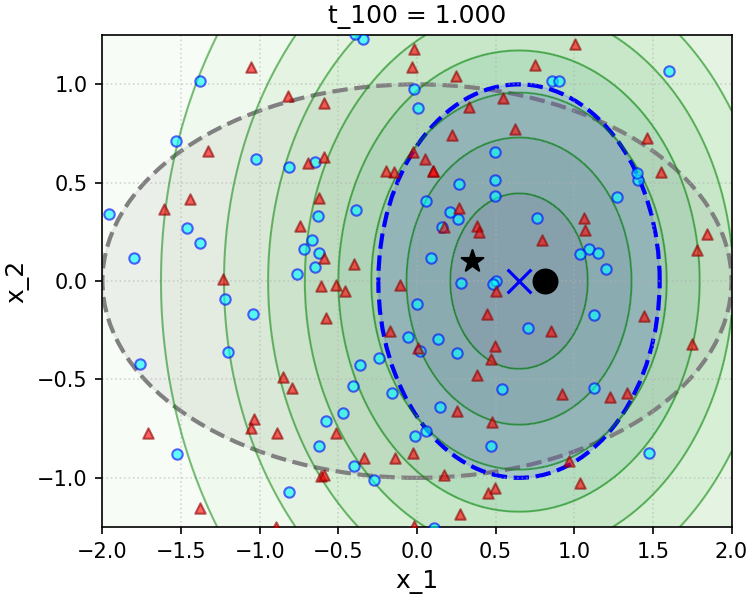
\includegraphics[width=\linewidth]{figs_chap5/samples_step_000_t_100_largenoise.png}
      % \caption{}
      % \label{}
    \end{subfigure}
    \hfill
    \begin{subfigure}{0.32\textwidth}
      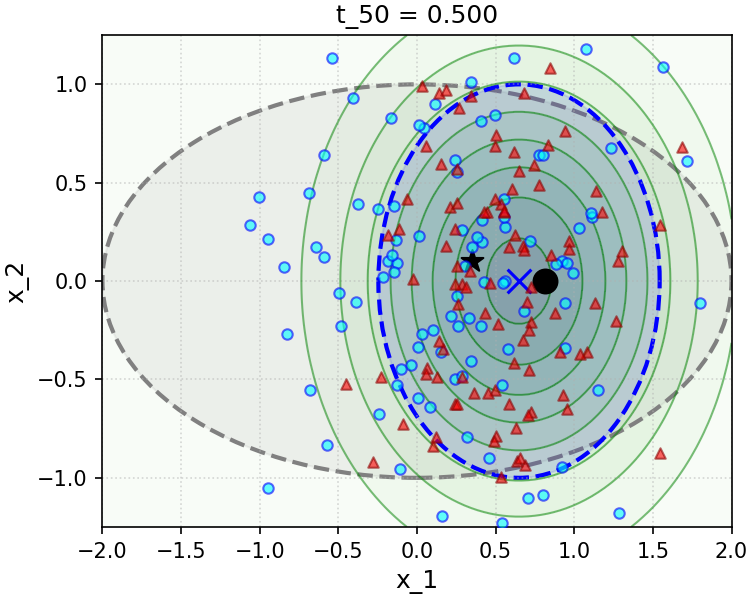
\includegraphics[width=\linewidth]{figs_chap5/samples_step_050_t_50_largenoise.png}
      % \caption{}
      % \label{}
    \end{subfigure}
    \hfill
    \begin{subfigure}{0.32\textwidth}
      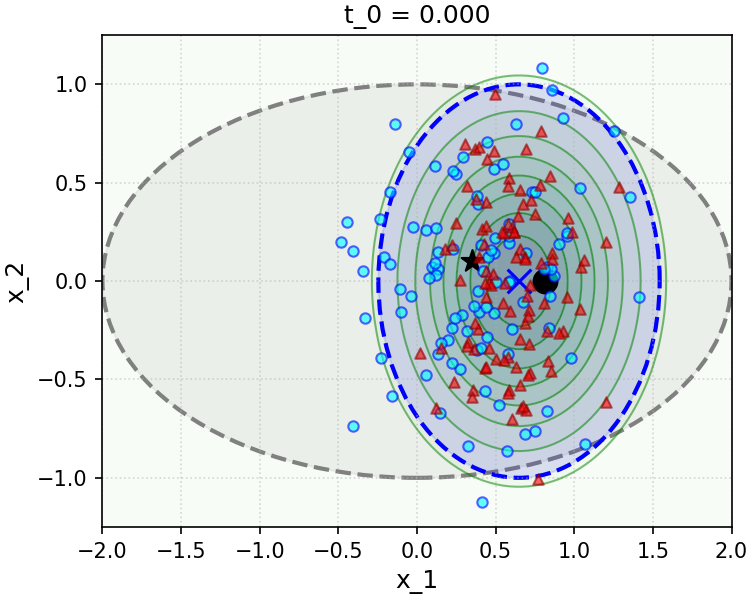
\includegraphics[width=\linewidth]{figs_chap5/samples_step_100_t_0_largenoise.png}
      % \caption{}
      % \label{}
    \end{subfigure}

    \vspace{2mm} % Add some vertical space between rows

    % Bottom row (3 images)
    \begin{subfigure}{0.32\textwidth}
      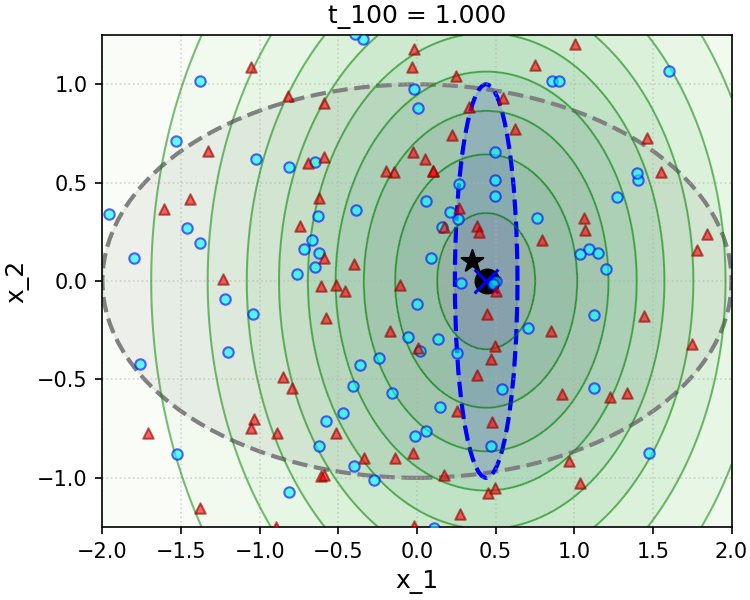
\includegraphics[width=\linewidth]{figs_chap5/samples_step_000_t_100_smallnoise.png}
      % \caption{}
      % \label{}
    \end{subfigure}
    \hfill
    \begin{subfigure}{0.32\textwidth}
      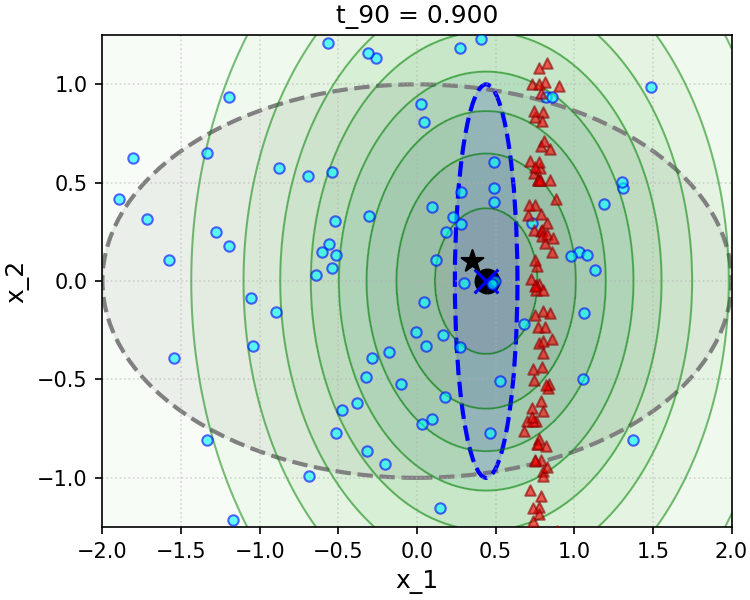
\includegraphics[width=\linewidth]{figs_chap5/samples_step_010_t_90_smallnoise.png}
      % \caption{}
      % \label{}
    \end{subfigure}
    \hfill
    \begin{subfigure}{0.32\textwidth}
      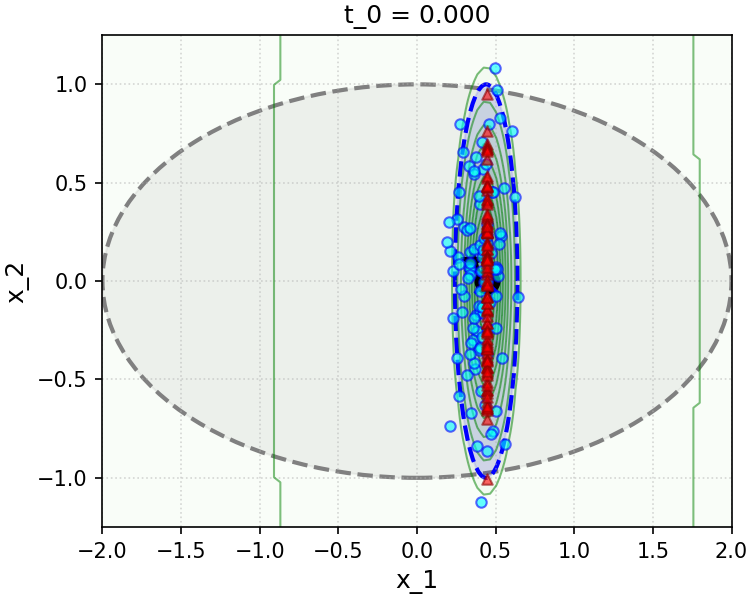
\includegraphics[width=\linewidth]{figs_chap5/samples_step_100_t_0_smallnoise.png}
      % \caption{}
      % \label{}
    \end{subfigure}

    \caption{Numerical simulation of the conditional sampling setup
    \eqref{eq:measurement-matching-observation}, with Gaussian data, linear
    measurements, and Gaussian noise. We simulate $D=2$ and $d=1$, with $\vSigma
    = \ve_1 \ve_1^\top + \tfrac{1}{4} \ve_2 \ve_2^\top$, $\vmu = \Zero$, and
    $\vA = \ve_1^\top$. The underlying signal $\vx$ is marked with a black star,
    and the measurement $\vy$ is marked with a black circle.
    Each individual plot corresponds to a different value of sampler time
    $t_{\ell}$, with different rows corresponding to different observation noise
    levels $\sigma^2$.
    In each plot, the covariance matrix of $\vx$ is plotted in gray, the
    posterior covariance matrix and posterior mean of $p_{\vx \mid \vy}$ are
    plotted in blue (with the posterior mean marked by a blue ``x''), and
    contours for $p_{\vx_{t_{\ell}} \mid \vy}$ are drawn in green. The sampler
    hyperparameters are $T=1$, $L=100$, and we draw $100$
    independent samples to initialize the samplers. Samplers are implemented
    with the closed-form denoisers derived in
    \Cref{example:denoising-conditional-gaussian}, with those using the
    approximation
    \eqref{eq:conditional-posterior-measurementmatching-gaussian-case-dps-approx}
    marked with red triangles, and those using the exact conditional posterior
    denoiser marked with blue circles.
    \textbf{Top:} For large observation noise $\sigma = 0.5$, both the exact
    conditional posterior denoiser and the approximate one do a good job of
    converging to the posterior $p_{\vx \mid \vy}$. Sampling time (corresponding
    to time in the ``forward process'', so larger times mean larger noise)
    decreases from left to right.  The convergence dynamics for the exact and
    approximate measurement matching term are similar. \textbf{Bottom:} For
    smaller observation noise $\sigma = 0.1$, the
    approximate measurement matching term leads to extreme bias in the sampler
    (red triangles): samples rapidly converge to an affine subspace
    of points that are consistent, modulo some shrinkage from the posterior mean
    denoiser, with the measured ground truth, and later sampling iterations are
    unable to recover the lost posterior variance along this dimension. Note
    that different times $t_{\ell}$ are plotted in the bottom row, compared to
    the top row, to show the rapid collapse of the approximation to the
    posterior along the measurement dimension.}
    \label{fig:conditional_sampling_computational_gaussian}
  \end{figure}

  \Cref{eq:conditional-posterior-measurementmatching-gaussian-case-dps-approx}
  is, of course, a direct consequence of our calculations above. However, notice
  that if we directly interpret this approximation, it is \textit{ab initio}
  tractable: the likelihood $p_{\vy \mid \vx} = \cN(\vA\vx, \sigma^2 \vI)$ is
  a simple Gaussian distribution centered at the observation, and the
  approximation to the measurement matching term that we arrive at can be
  interpreted as simply evaluating the log-likelihood at the conditional
  expectation $\bE[\vx \mid \vx_t = \vxi]$, then taking gradients with respect
  to $\vxi$ (and backpropagating through the conditional expectation, which is
  given here by \Cref{eq:posterior-denoiser-gaussian-case}).
  Nevertheless, note that the approximation in
  \Cref{eq:conditional-posterior-measurementmatching-gaussian-case-dps-approx}
  requires $t \ll \sqrt{\lambda_{\min}(\vSigma)}$, and that it is never accurate
  in general when this condition does not hold, even in this Gaussian setting.

  To gain insight into the effect of the convenient approximation
  \eqref{eq:conditional-posterior-measurementmatching-gaussian-case-dps-approx},
  we implement and simulate a simple numerical experiment in the Gaussian
  setting in \Cref{fig:conditional_sampling_computational_gaussian}. 
  The sampler we implement is a direct implementation of the simple scheme
  \eqref{eq:denoising-iteration-basic} we have developed in \Cref{ch:compression}
  and recalled above, using the true conditional posterior denoiser, i.e.\
  \Cref{eq:conditional-posterior-denoiser-gaussian-case} (top row of
  \Cref{fig:conditional_sampling_computational_gaussian}), and the 
  convenient approximation to this denoiser made with the decomposition
  \eqref{eq:posterior-sampling-denoiser-decomposition}, the posterior denoiser
  \eqref{eq:posterior-denoiser-gaussian-case}, and the measurement
  matching approximation
  \eqref{eq:conditional-posterior-measurementmatching-gaussian-case-dps-approx}
  (bottom row of \Cref{fig:conditional_sampling_computational_gaussian}).
  We see that even in the simple Gaussian setting, the approximation to the
  measurement matching term we have made is not without its
  drawbacks---specifically, at small noise levels $\sigma^2 \ll 1$, it leads to
  rapid collapse of the variance of the sampling distribution along directions
  that are parallel to the rows of the linear measurement operator $\vA$, which
  cannot be corrected by later iterations of sampling. We can intuit this from
  the approximation
  \eqref{eq:conditional-posterior-measurementmatching-gaussian-case-dps-approx}
  and the definition of the denoising iteration
  \eqref{eq:denoising-iteration-basic}, given
  \Cref{eq:posterior-sampling-denoiser-decomposition}: for $\sigma^2 \ll 1$,
  early steps of sampling effectively take gradient descent steps with a very
  large step size on the likelihood, via
  \Cref{eq:conditional-posterior-measurementmatching-gaussian-case-dps-approx},
  which leads the sampling distribution to get ``stuck'' in a collapsed state.

  % On the other hand, the second (more tractable) scheme in
  % \Cref{fig:posterior-sampling-cds}, which involves generating $\vx_t$ by adding
  % noise to $\vx$ and then conditioning on $\vy$ after, produces a different
  % joint distribution
  % \begin{equation}
  %   \begin{bmatrix}
  %     \vx \\
  %     \vx_t \\
  %     \vy
  %   \end{bmatrix}
  %   =_{d}
  %   \begin{bmatrix}
  %     \vSigma^{1/2} & \Zero & \Zero \\
  %     \vSigma^{1/2} & t\vI & \Zero \\
  %     \vA \vSigma^{1/2} & \Zero & \sigma \vI
  %   \end{bmatrix}
  %   \begin{bmatrix}
  %     \vg \\
  %     \vg' \\
  %     \vw
  %   \end{bmatrix}
  %   +
  %   \begin{bmatrix}
  %     \vmu \\
  %     \vmu \\
  %     \vA\vmu
  %   \end{bmatrix},
  % \end{equation}
  % where $\vg' \sim \cN(\Zero, \vI)$ independent of the other Gaussians.
  % This is again a jointly Gaussian distribution, with covariance
  % \begin{equation*}
  %   \begin{bmatrix}
  %     \vSigma^{1/2} & \Zero & \Zero \\
  %     \vSigma^{1/2} & t\vI & \Zero \\
  %     \vA \vSigma^{1/2} & \Zero & \sigma \vI
  %   \end{bmatrix}
  %   \begin{bmatrix}
  %     \vSigma^{1/2} & \Zero & \Zero \\
  %     \vSigma^{1/2} & t\vI & \Zero \\
  %     \vA \vSigma^{1/2} & \Zero & \sigma \vI
  %   \end{bmatrix}^\top
  %   =
  %   \begin{bmatrix}
  %     \vSigma & \vSigma & \vSigma\vA^\top \\
  %     \vSigma & \vSigma + t^2\vI & \vSigma\vA^\top \\
  %     \vA \vSigma & \vA\vSigma & \vA\vSigma\vA^\top + \sigma^2 \vI
  %   \end{bmatrix}.
  % \end{equation*}
  % Using \Cref{exercise:conditional_gaussian} once again, we derive the posterior
  % as
  % \begin{equation}
  %   p_{\vx \mid \vy, \vx_t}
  %   =
  %   \cN\left(
  %     ...
  %   \right)
  % \end{equation}
\end{example}

\Cref{example:denoising-conditional-gaussian} suggests a convenient
approximation for the measurement matching term
\eqref{eq:conditional-posterior-measurementmatching-gaussian-case-dps-approx},
which can be made beyond the Gaussian setting of the example. To
motivate this approximation in greater generality, notice that
by conditional independence of $\vy$ and $\vx_t$ given $\vx$, we can write
\begin{equation}
  p_{\vy \mid \vx_t}(\vnu \mid \vxi)
  =
  \int p_{\vy \mid \vx}(\vnu \mid \vxi') p_{\vx \mid \vx_t}(\vxi' \mid \vxi)
  \odif  \vxi'.
\end{equation}
Formally, when the posterior $p_{\vx\mid \vx_t}$ is a delta function centered at
its mean $\bE[\vx \mid \vx_t=\vxi]$, the approximation
\eqref{eq:conditional-posterior-measurementmatching-gaussian-case-dps-approx} is
exact. More generally, when the posterior $p_{\vx \mid \vx_t}$ is highly
concentrated around its mean, the approximation
\eqref{eq:conditional-posterior-measurementmatching-gaussian-case-dps-approx} is
accurate. This holds, for example, for sufficiently small $t$, which we saw
explicitly in the Gaussian setting of
\Cref{example:denoising-conditional-gaussian}.
Although the numerical simulation in
\Cref{fig:conditional_sampling_computational_gaussian} suggests that this
approximation is not without its caveats in certain regimes, it has proved to be
a reliable baseline in practice, after being proposed by Chung et al.\ as
``Diffusion Posterior Sampling'' (DPS) \cite{chung2023diffusion}.
In addition, there are even principled and generalizable approaches to improve it by
incorporating better estimates of the posterior variance (which turn out to be
exact in the Gaussian setting of \Cref{example:denoising-conditional-gaussian}),
which we discuss further in the end-of-chapter summary. 

Thus, with the DPS approximation, we arrive at the following approximation for
the conditional posterior denoisers $\bE[\vx \mid \vy, \vx_t]$, via
\Cref{eq:posterior-sampling-denoiser-decomposition}:
\begin{equation}
  \bE[ \vx \mid \vx_t=\vxi, \vy=\vnu]
  \approx
  \bE[\vx \mid \vx_t=\vxi] 
  + t^2 \nabla_{\vxi} \log p_{\vy \mid \vx}(\vnu \mid \bE[\vx \mid \vx_t = \vxi]).
  \label{eq:posterior-sampling-denoiser-decomposition-dps}
\end{equation}
And, for a neural network or other model $\bar{\vx}_{\theta}(t, \vxi)$ 
trained as in \Cref{sub:compression_denoising} to approximate the denoisers
$\bE[\vx \mid \vx_t = \vxi]$ for each $t \in [0, T]$, we arrive at the learned
conditional posterior denoisers
\begin{equation}
  \bar{\vx}_{\theta}(t, \vxi, \vnu) 
  = \bar{\vx}_{\theta}(t, \vxi)
  + t^2 \nabla_{\vxi} \log p_{\vy \mid \vx}(\vnu \mid \bar{\vx}_{\theta}(t,
  \vxi)).
  \label{eq:posterior-sampling-denoiser-learned-dps}
\end{equation}
Note that the approximation
\eqref{eq:posterior-sampling-denoiser-decomposition-dps} is  valid for arbitrary
forward models $h$ in the
observation model \eqref{eq:measurement-matching-observation}, including
nonlinear $h$, and even to
arbitrary noise models for which a clean expression for the likelihood $p_{\vy
\mid \vx}$ is known. Indeed, in the case of Gaussian noise, we have
\begin{equation}
  p_{\vy \mid \vx}(\vnu \mid \vxi)
  \propto
  \exp\left(
    -\frac{1}{2\sigma^2} \norm*{ h(\vxi) - \vnu }_2^2
  \right).
\end{equation}
Hence, evaluating the righthand side of
\eqref{eq:posterior-sampling-denoiser-learned-dps}
requires only
\begin{enumerate}
  \item A pretrained denoiser $\bar{\vx}_{\theta}(t, \vxi)$ for the data distribution $p$
    (of $\vx)$, learned as in \Cref{sub:compression_denoising} via
    \Cref{alg:learning_denoiser};
  \item Forward and backward pass access to the forward model $h$ for the
    measurements \eqref{eq:measurement-matching-observation};
  \item A forward and backward pass through $\bar{\vx}_{\theta}(t, \vxi)$, which can be evaluated
    efficiently using (say) backpropagation.
\end{enumerate}

\begin{algorithm}
  \caption{Conditional sampling under measurements
  \eqref{eq:measurement-matching-observation}, with an unconditional denoiser and DPS.}
	\label{alg:iterative_denoising_conditional}
	\begin{algorithmic}[1]
		\Require{An ordered list of timesteps \(0 \leq t_{0} < \cdots < t_{L} \leq T\) to use for sampling.}
    \Require{An unconditional denoiser \(\bar{\vx}_{\theta} \colon
    \{t_{\ell}\}_{\ell = 1}^{L} \times \R^{D} \to \R^{D}\) for $p_{\vx}$.}
    \Require{Measurement realization $\vnu$ of $\vy$ (\Cref{eq:measurement-matching-observation}) to condition on.}
    \Require{Forward model $h : \bR^D \to \bR^d$ and measurement noise variance
    $\sigma^2 > 0$.}
		\Require{Scale and noise level functions \(\alpha, \sigma \colon \{t_{\ell}\}_{\ell = 0}^{L} \to \R_{\geq 0}\).}
    \Ensure{A sample \(\hat{\vx}\), approximately from \(p_{\vy \mid \vx}\).}
    \Function{DDIMSamplerConditionalDPS}{$\bar{\vx}_{\theta}, \vnu, h, \sigma^2,
    (t_{\ell})_{\ell = 0}^{L}$}
		\State{Initialize \(\hat{\vx}_{t_{L}} \sim\) approximate distribution of \(\vx_{t_{L}}\)} \Comment{VP \(\implies \dNorm(\vzero, \vI)\), VE \(\implies \dNorm(\vzero, t_{L}^{2}\vI)\).}
		\For{\(\ell = L, L - 1, \dots, 1\)}
		% \State{Compute
		% 	\begin{equation*}
  %       \nabla_{\vxi}\left[ -\frac{1}{2\sigma^2} \norm*{h(
  %       \bar{\vx}_{\theta}(t_{\ell}, \vxi)
  %       ) - \vnu}_2^2 \right]\biggl|_{\vxi = \hat{\vx}_{t_{\ell}}}\biggr.
		% 	\end{equation*}
		% }
		\State{Compute
			\begin{equation*}
				\hat{\vx}_{t_{\ell - 1}} := \frac{\sigma_{t_{\ell
        - 1}}}{\sigma_{t_{\ell}}}\hat{\vx}_{t_{\ell}} + \bp{\alpha_{t_{\ell
        - 1}} - \frac{\sigma_{t_{\ell
        - 1}}}{\sigma_{t_{\ell}}}\alpha_{t_{\ell}}}\left(
        \bar{\vx}_{\theta}(t_{\ell}, \hat{\vx}_{t_{\ell}})
        - \frac{\sigma_{t_{\ell}}^2}{2\alpha_{t_\ell}\sigma^2}
        \nabla_{\vxi}\left[ \norm*{h( \bar{\vx}_{\theta}(t_{\ell}, \vxi)
        ) - \vnu}_2^2 \right]\biggl|_{\vxi = \hat{\vx}_{t_{\ell}}}\biggr.
        \right)
			\end{equation*}
		}
		\EndFor
		\State{\Return{\(\hat{\vx}_{t_{0}}\)}}
		\EndFunction
	\end{algorithmic}
\end{algorithm}

Combining this scheme with the basic implementation of unconditional sampling we
developed in \Cref{sub:compression_denoising}, we obtain a practical algorithm for
conditional sampling of the posterior $p_{\vx \mid \vy}$ given measurements
following \eqref{eq:measurement-matching-observation}.
\Cref{alg:iterative_denoising_conditional} records this scheme
for the case of
Gaussian observation noise with known standard deviation $\sigma$, with minor
modifications to extend to a general noising process, as in
\Cref{eq:gen_additive_gaussian_noise_model} and the surrounding discussion in
\Cref{ch:compression} (our discussion above made the simplifying choices $\alpha_t = 1$, $\sigma_t = t$, and
$t_{\ell} = T\ell / L$, as for \Cref{eq:denoising-iteration-basic} in
\Cref{sub:compression_denoising}).

% \sdb{The following is Yi's notes.}

% This problem is also known as the \href{https://arxiv.org/pdf/2209.14687}{Diffusion Posterior Sampling for General Noisy Inverse Problem}. 
% \yima{Below we follow the survey paper on conditional sampling:
% \href{https://arxiv.org/pdf/2410.00083}{A Survey on Diffusion Models
% for Inverse Problems}.}
% Now let us consider how to sample from the conditional distribution $p(\x\mid \y)$ given a measurement $\y = h(\x) + \vw$. From the Bayesian rule
% \
% we have:
% \begin{equation}
% \log p(\vx \mid \vy) = \log p(\vy \mid \vx) + \log p(\vx) - \log p(\vy).
% \label{eqn:Bayesian}
% \end{equation}
% Computing the gradient with respect to $\vx$, we have:
% \begin{equation}
% \nabla_{\vx} \log p(\vx \mid \vy) = \underbrace{\nabla_{\vx} \log
% p(\vy \mid \vx)}_{\text{measurement matching}} +
% \underbrace{\nabla_{\vx} \log p(\vx)}_{\text{score matching}}.
% \label{eqn:score-x}
% \end{equation}
% Notice that in the above expression, the second term is the {\em
% score matching} term introduced in Chapter \ref{ch:compression}. The
% first term here, known as the {\em measurement matching} term,
% produces a direction for $\vx$ in which the likelihood is higher for
% the observed $\vy$.

% \yima{Maybe give some representative examples for the measurement
% matching term where it has explicit formulae.}
% \begin{example}[Joint Gaussian Distribution]
% To build intuition, it is helpful to consider the important special case where
% $(\vx, \vy)$ are jointly Gaussian. Then $\vx$ and $\vy$ are necessarily
% (marginally) Gaussian, and moreover a standard calculation
% (Exercise \ref{exercise:conditional_gaussian}) shows that
% \begin{equation}
%   \vx \mid \vy \sim
% \end{equation}
% \end{example}

% \begin{example}[Linear Measurements]
% \label{eg:linear-measurement}
% Suppose the observation is linear:
% \begin{equation}
%     \y = h(\x) + \vw = \vA \vx + \vw, \quad \vw \sim \mathcal{N}(\mathbf{0}, \sigma^2
% \boldsymbol{I}).
% \end{equation}
% Then we have
% \begin{equation}
%    \nabla_{\vx} \log p(\vy \mid \vx) \propto \frac{1}{\sigma^2} \vA^\top(\y - \vA \x).  
% \end{equation}
% \end{example}

% Now if we want to learn and sample the condition distribution $p(\vx\mid \vy)$
% via the diffusion and denoising process $\vx_t$ and then sample from
% it, we have we have:
% \begin{equation}
% \nabla_{\vx_t} \log p(\vx_t \mid \vy) = {\nabla_{\vx_t} \log p(\vy
% \mid \vx_t)} + {\nabla_{\vx_t} \log p(\vx_t)}.
% \label{eqn:score-xt}
% \end{equation}

% \paragraph{Compute measurement matching.}
% In Chapter \ref{ch:compression}, we have shown how the score matching term ${\nabla_{\vx_t}
% \log p(\vx_t)}$ can be estimated and computed, when the diffusion process is Gaussian. Hence, we only need to find out how to compute the measurement matching term: $\nabla_{\vx_t} \log p(\vy \mid \vx_t)$. 

% Notice that in general, we only know the relationship between $\y$ and $\x$. By the construction of the diffusion process $\x_t$, we also know $\y$ is conditionally independent of $\x_t$, given $\x$. Hence we have:
% \begin{eqnarray}
%     p(\y \mid \x_t) &=& \int p(\y\mid \x, \x_t) p(\x\mid \x_t) \odif \x\\
%     &=& \int p(\y\mid \x) p(\x\mid \x_t) \odif \x.
% \end{eqnarray}
% Notice that the last equality is taking the expectation of $p(\y \mid \x)$, as a function of $\x$, with respect to the distribution $\x \sim p(\x \mid \x_t)$. 

% Under natural conditions, we may approximate the above expectation of a function of $\x$ as a function of its expectation $\bar{\x}(\x_t) = \int \x p(\x\mid \x_t) \odif \x$. Therefore, we have:
% \begin{eqnarray}
%     p(\y \mid \x_t)\approx  p(\y \mid \hat{\x}(\x_t)).
% \end{eqnarray}
% We then can approximately compute the measurement matching term: $\nabla_{\vx_t} \log p(\vy \mid \vx_t)$ as
% \begin{equation}
%    \nabla_{\vx_t} \log p(\vy \mid \vx_t) \approx \nabla_{\hat{\vx}} \log p(\vy \mid \hat{\x}) \nabla_{\vx_t} \hat{\x}(\x_t).
% \end{equation}
% Notice that the second derivative $\nabla_{\vx_t} \hat{\x}(\x_t)$ can be computed via backpropagation if the expectation $\hat{\x}(\x_t)$ is computed via a forward deep network, as did in Chapter \ref{ch:compression}. The first derivative $\nabla_{\hat{\vx}} \log p(\vy \mid \hat{\x})$ can be easily computed if an explicit measurement model is given, as in Example \ref{eg:linear-measurement}. If not, the conditional probability $p(\y\mid \x)$ is usually modeled by a deep network, say a classification network. Then the derivative can be evaluated via backpropagation through this network, again. 

% \paragraph{Iterative sampling via score matching and measurement matching.} 
% We now work the above conceptual derivation into the iterative denoising and sampling process for a practical algorithm that produces a sample based on the conditional distribution $\x \sim p(\x\mid \y)$.

\subsection{Conditional Sampling of General Paired Data}\label{sub:cfg}

In the previous section, we have seen how to use the denoising-diffusion
paradigm for conditional sampling from the posterior $p_{\vx \mid \vy}$ given
\textit{model-based} measurements $\vy = h(\vx) + \vw$
(\Cref{eq:measurement-matching-observation}), culminating in the
DPS algorithm \Cref{alg:iterative_denoising_conditional}. This is a powerful
framework, but there are many practical applications, especially in computer
vision and natural language processing, where an explicit generative model $h$
for the measurements/observations $\vy$ is not available due to the
intractability of analytical modeling. The most natural instance of this is
a classification problem, where $\vy$ represents the class label for
high-dimensional data $\vx$ (for example, a $224 \times 224$ RGB image from the
ImageNet dataset). In this section, we will present techniques for extending
conditional sampling to this setting.

Thus, we now assume only that we have access to samples from the joint
distribution of $(\vx, \vy)$:
\begin{equation}
  (\vx, \vy) \sim p_{\vx, \vy}.
\end{equation}
Our goal remains to produce conditional samples $\hat{\vx}$ from the posterior,
given realizations $\vnu$ of $\vy$:
\begin{equation}
  \hat{\vx} \sim p_{\vx \mid \vy}(\spcdot \mid \vnu).
\end{equation}
As in the previous section, we will repeatedly use the notation $\vxi$ to denote
realizations of $\vx$, and we define $\vx_t = \alpha_t \vx + \sigma_t \vg$
with $\vg \sim \cN(\Zero, \vI)$ independent of $(\vx, \vy)$, as in
\Cref{eq:gen_additive_gaussian_noise_model} in \Cref{ch:compression}.
To proceed, we note that our development of conditional sampling under
measurements \eqref{eq:measurement-matching-observation} did not explicitly use
the forward model $h$ except for in making the DPS approximation
\eqref{eq:conditional-posterior-measurementmatching-gaussian-case-dps-approx}.
In particular, we always have the conditional posterior denoiser decomposition
\eqref{eq:posterior-sampling-denoiser-decomposition} by virtue of Bayes' rule
and conditional independence of $\vy$ and $\vx_t$ given $\vx$ (recall
\Cref{fig:posterior-sampling-cds}), and thus we can
still write given only paired data $(\vx, \vy) \sim p_{\vx, \vy}$
\begin{equation}\label{eq:conditional-denoising-mmse-denoiser-paired-data}
  \bE[ \vx \mid \vx_t=\vxi, \vy=\vnu]
  =
  \bE[\vx \mid \vx_t=\vxi] + \frac{\sigma_t^2}{\alpha_t} \nabla_{\vxi}\log p_{\vy \mid \vx_t}(\vnu\mid
  \vxi).
\end{equation}
A natural ideal is then to directly implement the likelihood correction term in
\eqref{eq:conditional-denoising-mmse-denoiser-paired-data} using a deep network
$f_{\theta}$:
the network maps noisy data samples $\vx_t$ to a probability distribution over
measurements $\vy$, then one evaluates its gradient with respect to $\vx_t$
using backpropagation to compute the correction term in
\Cref{eq:conditional-denoising-mmse-denoiser-paired-data}.
Such an approach was already recognized and exploited to perform conditional
sampling in pioneering early works on diffusion models, notably those by
\citet{Sohl-Dickstein2015} and by \citet{song2020score}. For example, in the
setting where $\vy$ corresponds to a class label taking values in the index set
$\set{1, \dots, K}$, a deep network mapping noisy
inputs and their corresponding noise levels $(\vx_t, t) \in \bR^{D} \times
\bR$ to a probability distribution over labels $y \in \set{1, \dots, K}$ can be
trained via the standard cross entropy training with a labeled dataset by adding
independent noise to the training images.\footnote{In \Cref{ch:applications}, we
discuss the process of training such a classifier in full detail.}

However, this straightforward methodology has two key drawbacks. The first is
that, empirically, such a trained deep network classifier frequently does not
provide a strong enough guidance signal (in
\Cref{eq:conditional-denoising-mmse-denoiser-paired-data}) to ensure that
generated samples reflect the conditioning information $\vy$. This was first
pointed out by \citet{Dhariwal2021-hg}, who noted that in the setting of
class-conditional ImageNet generation, the learned deep network
classifier's probability outputs for the class $y$ being conditioned on were
frequently around
$0.5$---large enough to be the dominant class, but not large enough to provide
a strong guidance signal---and that upon inspection, generations were not
consistent with the conditioning class $y$. \citet{Dhariwal2021-hg} proposed to
address this heuristically by incorporating an ``inverse temperature''
hyperparameter $\gamma > 0$
into the definition of the conditional denoiser
\eqref{eq:conditional-denoising-mmse-denoiser-paired-data}:
\sdb{TODO: Not an equality...}
\begin{equation}\label{eq:denoiser-classifier-guidance}
  \bE[ \vx \mid \vx_t=\vxi, \vy=\vnu]
  =
  \bE[\vx \mid \vx_t=\vxi] 
  + \gamma\frac{\sigma_t^2}{\alpha_t} \nabla_{\vxi}\log p_{\vy \mid \vx_t}(\vnu\mid
  \vxi),
\end{equation}
with the case $\gamma = 1$ coinciding with
\eqref{eq:conditional-denoising-mmse-denoiser-paired-data}.
\citet{Dhariwal2021-hg} found that a setting $w > 1$ performed best empirically.
Note that
\begin{align}
  \gamma\frac{\sigma_t^2}{\alpha_t} \nabla_{\vxi}\log p_{\vy \mid \vx_t}(\vnu\mid
  \vxi)
  &=
  \frac{\sigma_t^2}{\alpha_t} \nabla_{\vxi}\log \left(
  p_{\vy \mid \vx_t}(\vnu\mid \vxi)^\gamma
  \right), %\\
  % &=
  % \frac{\sigma_t^2}{\alpha_t} \nabla_{\vxi}\log \left(
  % \frac{
  %   p_{\vy \mid \vx_t}(\vnu\mid \vxi)^w
  % }{
  %   \int p_{\vy \mid \vx_t}(\vnu'\mid \vxi)^w \odif \vnu'
  % }
  % \right)
\end{align}
which suggests the natural interpretation of the parameter $\gamma$ performing
(inverse) \textit{temperature scaling} on the likelihood
$p_{\vy \mid \vx_t}$, which is precise if we consider the renormalized
distribution 
$ { p_{\vy \mid \vx_t}(\vnu\mid \vxi)^\gamma } / { \int p_{\vy \mid \vx_t}(\vnu'\mid
\vxi)^\gamma \odif \vnu' } $.
However, note that this \textit{is not} a rigorous interpretation in the context
of \Cref{eq:conditional-denoising-mmse-denoiser-paired-data}, because the
gradients are taken with respect to $\vxi$, and the normalization constant in
the temperature-scaled distribution is in general a function of $\vxi$.
We will return to this point \sdb{in a subsequent example}.
Regardless, choosing $\gamma > 1$ has the effect of exaggerating large values of the
likelihood $p_{\vy \mid \vx_t}$ relative to smaller ones, which amplifies the
guidance signal provided, leading to dramatic improvements in generation quality
and faithfulness to the conditioning signal in practice.

% \begin{example}[Classification] One may view the problem of
% classification as a special case for completing or predicting
% missing parts of a random vector. For classification, given a
% sample vector $\x$, we would like to predict its class label $\y$.
% If we stack the two together as one joint vector:
% \begin{equation}
%   \vw = (\x, \y),
% \end{equation}
% one may view the problem of predicting the class label $\y$ as a
% problem of completing $\vw$ by observing only the $\x$ part. This
% is usually done by estimating and transforming the joint
% distribution of $\vw$ that minimizes the entropy (or coding
% rate) of the resulting representation of the empirical distribution
% of $\vx$.\footnote{A set of samples for $\x$ and their associated
% class labels $\y$} In fact, the common practice of introducing an
% auxiliary ``class token'' in the training of a Transformer for
% classification tasks can be viewed as learning such a
% representation by compressing (the coding rate of) given samples of
% $\vw$. If the distribution of the data $\x$ is already a
% mixture of (low-dimensional) Gaussians, the work
% \cite{wright2008classification} showed that classification can be
% done effectively by directly minimizing {\em the (lossy) coding
% length} associated with the given samples.
% \end{example}

Nevertheless, classifier guidance does not address the second key drawback of
our straightforward methodology: it is both cumbersome and wasteful to have to
train an auxiliary classifier in addition to the denoisers $\bE[\vx \mid
\vx_t]$, given that it is not possible to directly adapt a pretrained classifier
due to the need for it to work well on noisy inputs $\vx_t$ and take the time
$t$ as input. \citet{Dhariwal2021-hg} found that it was necessary to explicitly
design the architecture of the deep network implementing the classifier to match
that of the denoiser, which motivated \citet{Ho2022-ry} to propose a more
unified methodology, known as classifier-free guidance (CFG). \sdb{CFG...}

\sdb{Maybe cite Dieleman blog here (very quality). Cite preetum's paper as
necessary for understanding.}

\begin{example}
  \sdb{TODO: CG and CFG in the context of the mixture of gaussian example...
  from Ch3... cite yuchen wu paper...}
\end{example}

\sdb{Cross attention connection: slight generalization of the previous
``measurement'' example, relevant to CFG parameterization of networks. The
previous example leads naturally into this discussion. Mention ControlNet.}

% In practice, there are typically two situations:
% one is that the observation function $h(\spcdot)$ is explicitly known,
% and the other is when $h(\spcdot)$ is not known but only samples of the
% joint distribution $p(\vx, \vy)$ are given.
% Two representative subclasses of these settings worth keeping in mind are:
% \begin{enumerate}
%   \item \textbf{Known $h$: Analytically-Structured Observations.} 
%     Like image/matrix completion, we
%     are often faced with a setting where $\vy$ denotes a degraded or otherwise
%     ``lossy''
%     observation of the input $\vx$. This can manifest in quite different
%     forms. For example, in various scientific or
%     medical imaging problems, the measured data $\vy$ may be a compressed and
%     corrupted observation of the underlying data $\vx$; whereas in 3D vision tasks,
%     $\vy$ may represent an image captured by a camera of a physical object with an
%     unknown (low-dimensional) pose $\vx$ \sdb{TODO: verify}.
%     Generally, by virtue of mathematical modeling (and, in some cases, co-design
%     of the measurement system), we know $h$, and can exploit this knowledge to help
%     reconstruct or sample $\vx$.
%   \item \textbf{Paired Samples $(\vx, \vy)$: Controllable Generation.} In more
%     general applications such as computer vision or natural language processing
%     on internet-scale datasets,
%     it is common for data $\vx$, say images or texts, to have known
%     \textit{attributes} that we want to use for controllable sampling of the
%     data distribution. In these cases,
%     the analytical relationship between the data $\vx$ and its attributes $\vy$
%     is intractable to model, but we may still proceed by exploiting the
%     statistical relationship between the paired samples $(\vx, \vy)$.
%     We will illustrate this setting with detailed vignettes from vision,
%     where, for example, $\vy$ represents a text caption or a segmentation mask
%     for an image $\vx$.
% \end{enumerate}
% The attentive reader may ask why we need to study the first class of scenarios,
% given that it is technically a special case of the latter. We will see later,
% both in theory and in practice, that exploiting knowledge of $h$ can lead to
% superior performance.



\subsection{Applications for Conditional Generation}\label{sub:conditional-apps}
Below we give some vignettes for solving several typical
conditional sampling problems with the diffusion/denoising method,
including the previous image-completion problem. For different
applications, in practice, the measurement-matching term could be
introduced into the (iterative denoising) deep architecture by 
different means.

\subsubsection{Image Completion}
\yima{I believe Jong Chul Ye has some work \href{https://arxiv.org/pdf/2209.14687}{Diffusion Posterior Sampling for General Noisy Inverse Problem} along the same line of thought which is more principled, following the above measurement-matching approach... We could feature that work here. Also, we should mention that the work of \cite{wei2023diffusion} has shown how to use transformer-like architecture to realize diffusion/denoising
models for image completion
(\href{https://weichen582.github.io/diffmae.html}{Diffusion Models as
Masked Autoencoders}). However, the realization of conditional sampling is somewhat heuristic.}

\subsubsection{Conditional Pose Prediction}
Another good example of denosing/diffusion based conditional sampling
is Brent's recent work on body gesture estimation conditioned on the
head pose (\href{https://egoallo.github.io}{Estimating Body and Hand
Motion in an Ego-sensed World}).\yima{Brent Yi better straighten out his work on pose estimation in the above context of conditional sampling... }

\subsubsection{Conditional Image Generation}
\sdb{Align Visual Data with Texts, ControlNet, ... discuss dhariwal and nichol
(classifier aware guidance), then mention DALLE type architecture for
text-conditioned image generation?} \yima{Actually the original work ``\href{https://arxiv.org/abs/2105.05233}{Diffusion Models Beat GANs on Image Synthesis}'', by Prafulla Dhariwal and Alex Nichol, proposed to compute the two matching functions proposed above. The follow-up work ``Classifer-Free Diffusion Guidance''  by
Jonathan Ho and Tim Salimans tried to simplify this by training the two matching functions together with one network with different condition inputs. We should feature those works here. However, we can mention that the large-scale realization DALLE, with a learned joint image-text binding by CLIP, adopts a somewhat heuristic way to realize the conditioning. So were many other follow-up works such as the ControlNet etc. ...}

\section{Summary and Notes}
Scalability of the masked autoencoding (MAE) or the masked
autoencoding via diffusion (MAD).

Potentially a better diffusion or conditional diffusion  with a CRATE backbone?


% SAM: Commenting this out while we still have this section rendering
% \paragraph{Shallow vs.\ deep neural networks, for autoencoding and more.}
% In \Cref{sub:nonlinear-pca}, we discussed Cybenko's universal approximation
% theorem and how it states that in principle, a neural network with a single
% hidden layer (and suitable elementwise nonlinearities) is sufficient to
% approximate any suitably regular target function. Of course, in practice, the
% major architectural reason for the dominance of neural networks in practice has
% been the refinement of techniques for training \textit{deeper} neural networks.
% Why is depth necessary?
% From a fundamental point of view, the issue of depth separations, which
% construct settings where a deeper neural network can approximate a given class
% of target functions with exponentially-superior efficiency relative to a shallow
% network,
% has been studied at great length in the theoretical literature:
% examples include \cite{Telgarsky2016-sn,Bresler2020-xy,Venturi2021-qc}. 
% The ease of training deeper
% networks in practice has not received as satisfying of an answer from the
% perspective of theory. 
% ResNets \cite{he2016deep} represent the pioneering empirical work of
% making deeper networks more easily trainable, used in nearly all modern
% architectures in some form. Theoretical studies have focused heavily on
% trainability of very deep networks, quantified via the initial neural tangent
% kernel \cite{Buchanan2021-sj,Martens2021-cx}, but these studies have not given
% significant insight into the trainability benefits of deeper networks in middle
% and late stages of training (but see \cite{Yang2021-gw} for the root of a line
% of research attempting to address this).

\paragraph{Measurement matching without clean samples.} In our development of
conditional sampling, we considered measurement matching under an observation
model \eqref{eq:measurement-matching-observation}, where we assume that we have
paired data $(\vx, \vy)$---i.e., ground truth for each observation $\vy$.
In many practically-relevant inverse problems, this is not the case: one of the
most fundamental examples is in the context of compressed sensing, which we
recalled in \Cref{ch:classic}, where we need to reconstruct $\vx$ from $\vy$
using prior knowledge about $\vx$ (i.e., sparsity).
In the setting of denoising-diffusion, we have access to an implicit prior for
$\vx$ via the learned denoisers $\bar{\vx}_{\theta}(t, \vxi)$. Can we still perform 
conditional sampling without access to ground truth samples $\vx$?

For intuition as to why this might be possible, we recall a classical example
from statistics known as Stein's unbiased risk estimator (SURE).
Under an observation model $\vx_t = \vx + t \vg$ with $\vg \sim \cN(\Zero,
\vI)$ and $t>0$, it turns out that for any weakly differentiable $f : \bR^D \to \bR^D$,
\begin{equation}\label{eq:sure-risk}
  \bE_{\vg}\left[
    \norm*{\vx - f(\vx + t \vg)}_2^2
    \right]
  =
  \bE_{\vg}\left[
    \norm*{\vx+t\vg - f(\vx + t \vg)}_2^2
    + 2t^2 \nabla \cdot f(\vx + t\vg)
    \right]
  - t^2 D,
\end{equation}
where $\nabla \cdot$ denotes the divergence operator:
\begin{equation*}
	\nabla \cdot f = \sum_{i=1}^D \partial_i f_i.
\end{equation*}
The $\vx$-dependent part of the RHS of \Cref{eq:sure-risk} is called Stein's unbiased risk
estimator (SURE). If we take expectations over $\vx$ in \Cref{eq:sure-risk},
note that the RHS can be written as an expectation with respect to $\vx_t$---in
particular, the mean-squared error of \textit{any denoiser $f$} can be estimated
\textit{solely from noisy samples}!
This remarkable fact, in refined forms, constitutes the basis for many practical
techniques for performing image restoration, denoising-diffusion, etc.\ using
only noisy data: notable examples include the ``noise2noise'' paradigm
\cite{pmlr-v80-lehtinen18a}
and Ambient Diffusion \cite{daras2023ambient}.

As a fun aside, we point out that \Cref{eq:sure-risk} leads to an alternate
proof of Tweedie's formula (\Cref{thm:tweedie}). At a high level, one takes
expectations over $\vx$ and expresses the main part of the RHS of
\Cref{eq:sure-risk} equivalently, via integration by parts, as
\begin{equation}
  \bE_{\vx_t}\left[
    \norm*{\vx_t - f(\vx_t)}_2^2
    + 2t^2 \nabla \cdot f(\vx_t)
    \right]
  =
  \bE_{\vx_t}\left[
    \norm*{\vx_t - f(\vx_t)}_2^2
    \right]
  - 2t^2 \int
  \ip*{\nabla p_{\vx_t}(\vxi)}{f(\vxi)}
  \odif \vxi.
\end{equation}
This is a quadratic function of $f$, and formally taking derivatives gives
that the optimal $f$ satisfies Tweedie's formula (\Cref{thm:tweedie}). This
argument can be made rigorous using basic ideas from the calculus of variations.


\paragraph{Corrections to the Diffusion Posterior Sampling (DPS) approximation.}
In \Cref{example:denoising-conditional-gaussian} and in particular in
\Cref{fig:conditional_sampling_computational_gaussian}, we pointed out
a limitation of the DPS approximation
\Cref{eq:conditional-posterior-measurementmatching-gaussian-case-dps-approx} at
small levels of measurement noise. 
This limitation is well-understood, and a principled approach to ameliorating it
has been proposed by Rozet et al.\ \cite{rozet2024learning}.
The approach involves incorporating an additional estimate for the variance of
the noisy posterior $p_{\vx \mid \vx_t}$ to
\Cref{eq:conditional-posterior-measurementmatching-gaussian-case-dps-approx}---we
refer to the paper for details.
Natural estimates for the posterior variance are slightly less scalable than DPS
itself, due to the need to invert an affine transformation of the Jacobian of
the posterior denoiser $\bE[\vx \mid \vx_t=\vxi]$ (a large matrix). This is done
relatively efficiently by Rozet et al.\ \cite{rozet2024learning} using autodifferentiation and an
approximation for the inverse based on conjugate gradients. It seems that it
should be possible to improve further over this approach (say, using classical
ideas from second-order optimization).


\paragraph{More about measurement matching and diffusion models for inverse
problems.} 

Diffusion models have become an extremely popular tool for solving inverse
problems arising in scientific applications. Many more methods beyond the simple
DPS algorithm we have presented in \Cref{sub:measurement-matching} have been
developed and continue to be developed, as the area is evolving rapidly.
Popular and performant classes of approaches beyond DPS, which we have presented
due to its generality, include variable splitting approaches like DAPS
\cite{Zhang2024-ha},
which allow for specific measurement constraints to be enforced much more
strongly than in DPS, and exact approaches that can avoid the use of
approximations like in DPS, such as TDS \cite{wu2023practical}.
For more on this area, we recommend \cite{zheng2025inversebench}, which
functions simultaneously as a survey and a benchmark of several popular methods
on specific scientific inverse problem datasets.

\section{Exercises and Extensions}





\end{document}
